\documentclass[]{article}
\usepackage{caption,subcaption,graphicx,float,url,amsmath,amssymb,tocloft}
\usepackage[hidelinks]{hyperref}
\usepackage[toc,acronym,nonumberlist]{glossaries}
\setacronymstyle{long-short}
\usepackage{glossaries-extra}
\graphicspath{{figs/}} 
\setlength{\cftsubsecindent}{0em}
\setlength{\cftsecnumwidth}{3em}
\setlength{\cftsubsecnumwidth}{3em}

%opening
\title{
	Notes from Origins of Life\\
	Week 6: Astrobiology \& General Theories of Life
}
\author{Simon Crase}

\makeglossaries
\renewcommand{\thesection}{6.\arabic{section}}

\loadglsentries{glossary-entries}

\renewcommand{\glstextformat}[1]{\textbf{\em #1}}

\begin{document}

\maketitle

\begin{abstract}
   These are my notes from the $6^{th}$ Week of the Santa Fe Institute Origins of Life Course\cite{sfi2019}. The course aims to push the field of Origins of Life research forward by bringing new and synthetic thinking to the question of how life emerged from an abiotic world.\\
   The content and images contained herein are the intellectual property of the Santa Fe Institute, with the exception of any errors in transcription, which are my own.
   These notes are distributed in the hope that they will be useful,
   but without any warranty, and without even the implied warranty of
   merchantability or fitness for a particular purpose. All feedback is welcome,
   but I don't necessarily undertake to do anything with it.

\end{abstract}

\setcounter{tocdepth}{2}
\tableofcontents

\listoffigures

\section{Introduction}

Lecturer: Chris Kempes

Ultimate goal is to provide a general theory of Life, one capable of uncovering the history we know about, but also bounding the possibilities for other types of life, and helping us recognize other forms of life. In this unit we'll discuss the search for life beyond Earth and how origins of life fits into this effort. We'll also discuss general evolutionary processes and abstract life. 

\section{Origins of Life and Astrobiology}

Lecturer: Sara Imari Walker

Why is Origins so important to Astrobiology? We want to be able to identify living organisms on another planet. We can send robotic missions within the Solar System, but we have only a small amount of data for exoplanets.

 What makes worlds with life different--Figure \ref{fig:Jupiter:Tellus}? Jupiter and Earth both have non-equilibrium surface features, so that isn't sufficient.

\begin{figure}[H]
	\caption{What makes worlds with life different?}\label{fig:Jupiter:Tellus}
	\begin{subfigure}[b]{0.45\textwidth}
		\caption{Jupiter}\label{fig:Jupiter}
		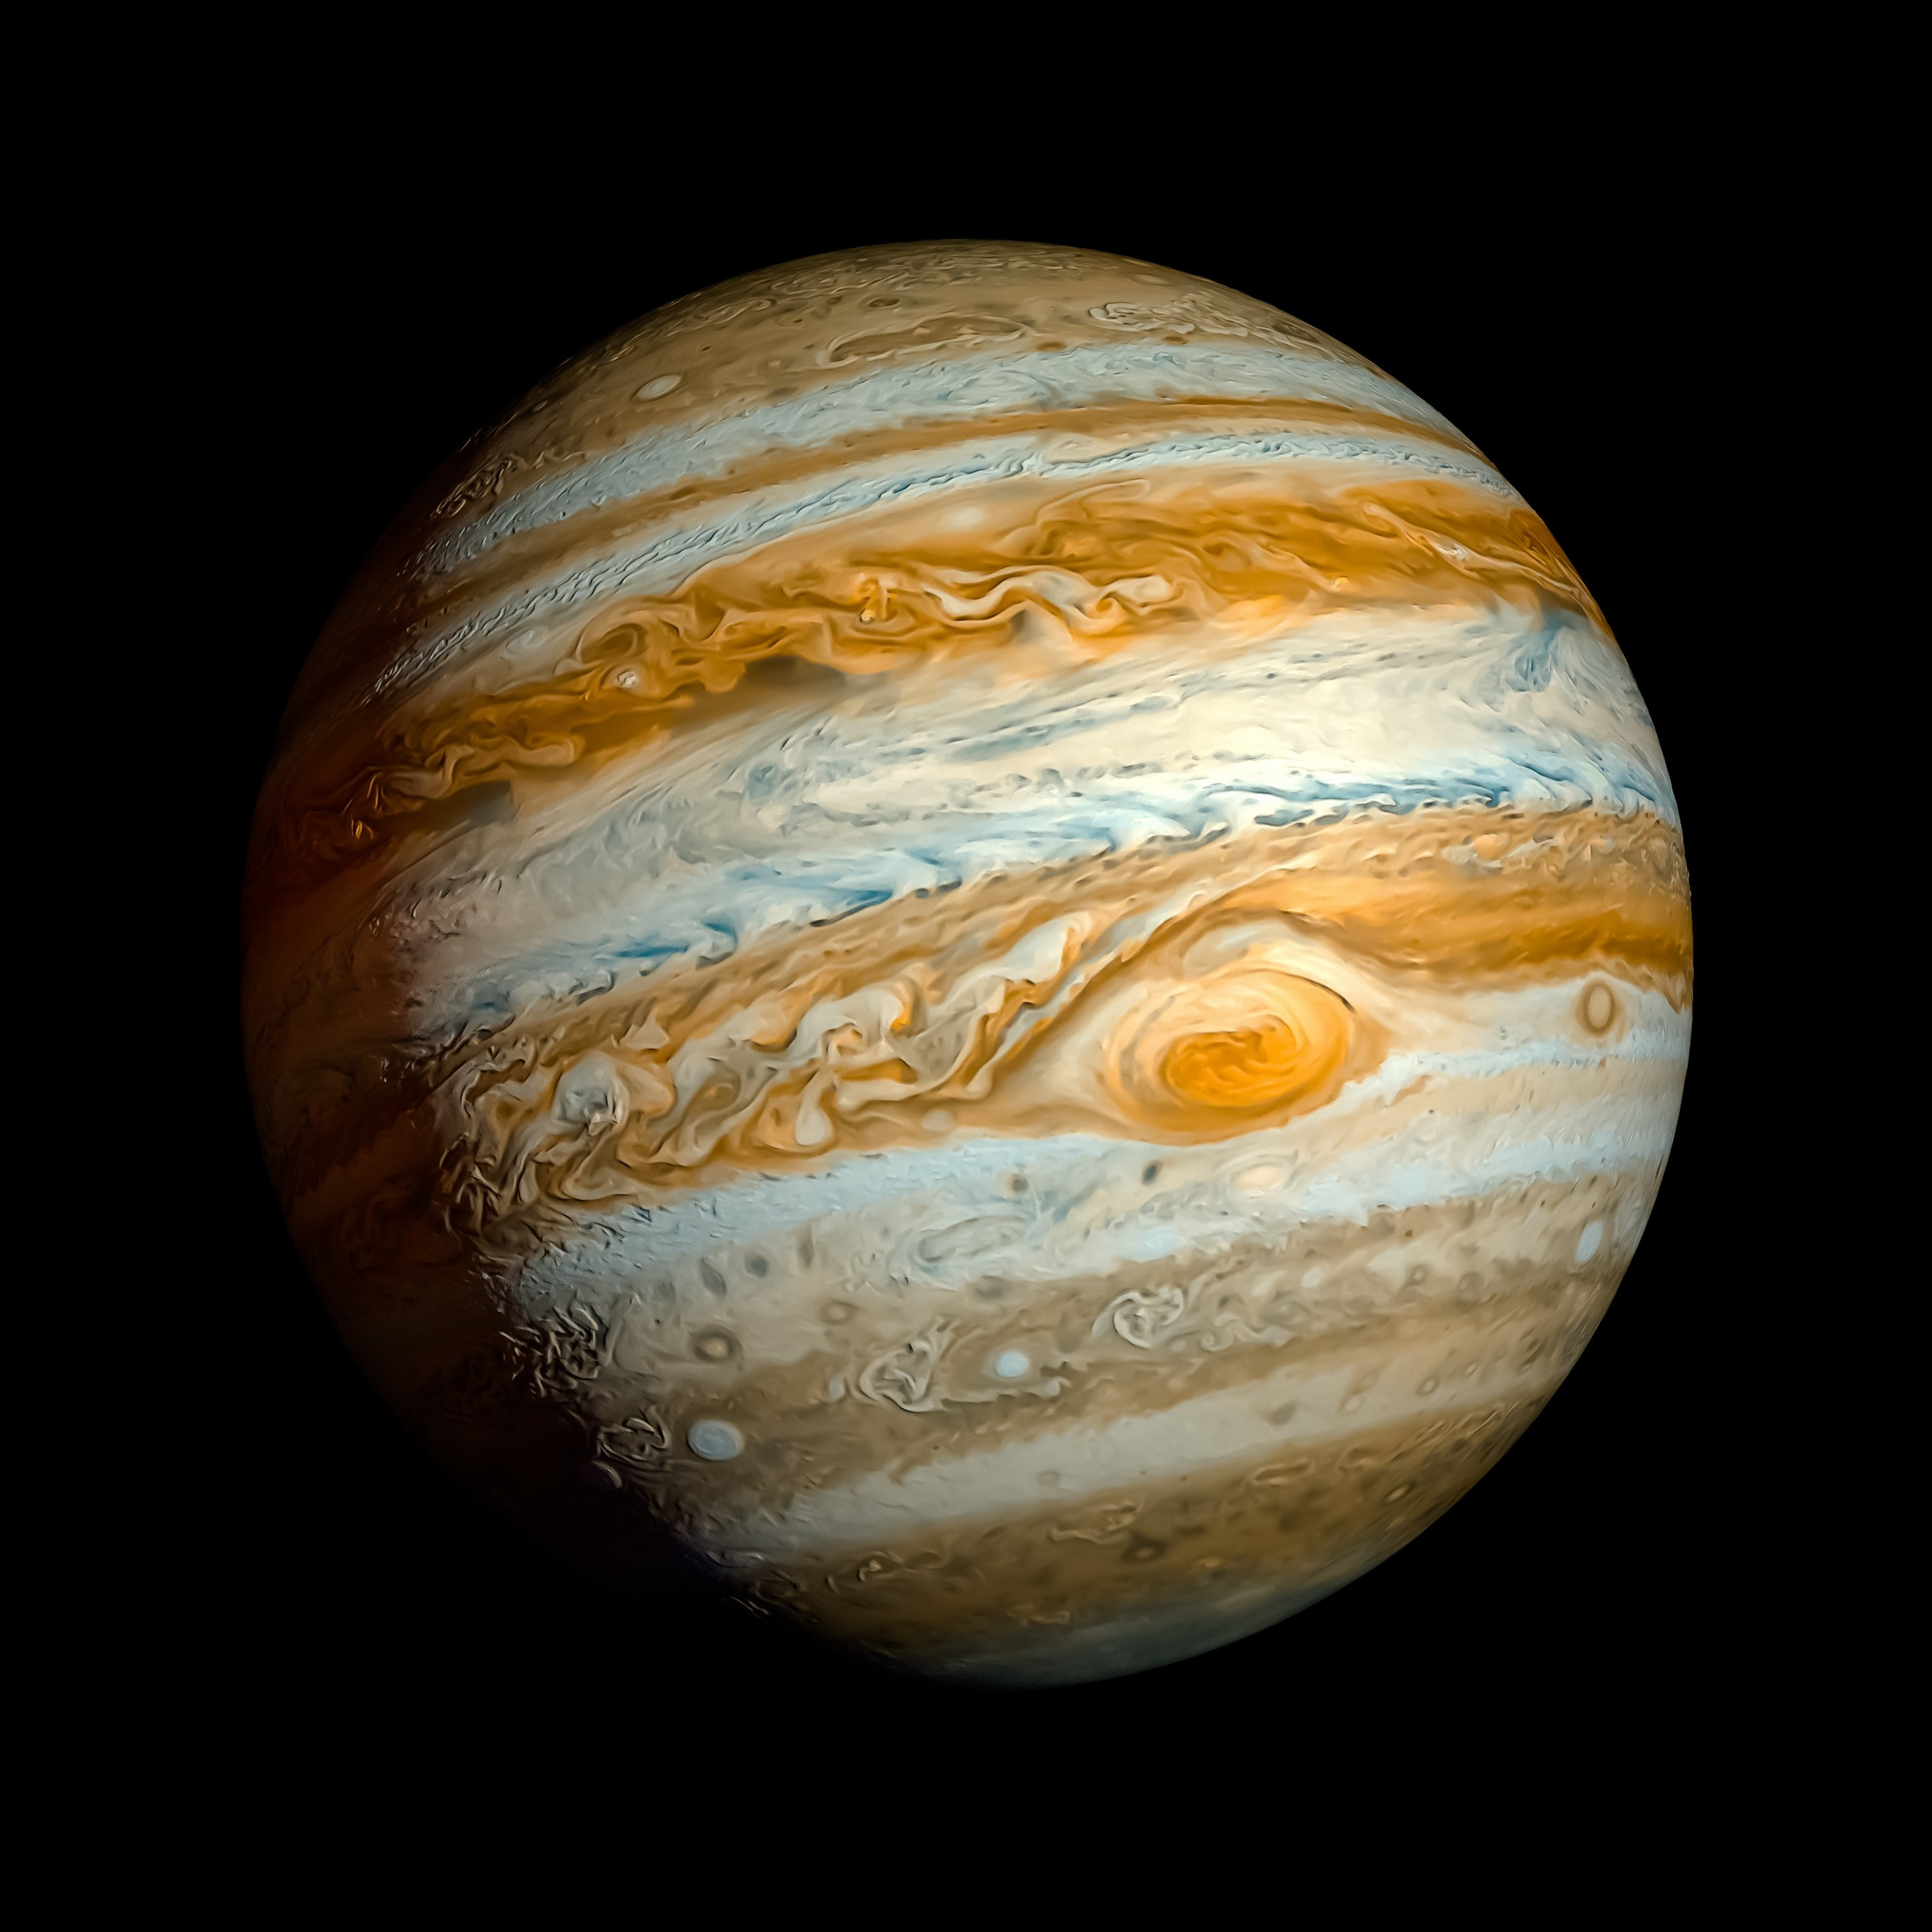
\includegraphics[width=\textwidth]{Jupiter}
	\end{subfigure}
	\begin{subfigure}[b]{0.45\textwidth}
		\caption{Earth at night}\label{fig:Earth}
		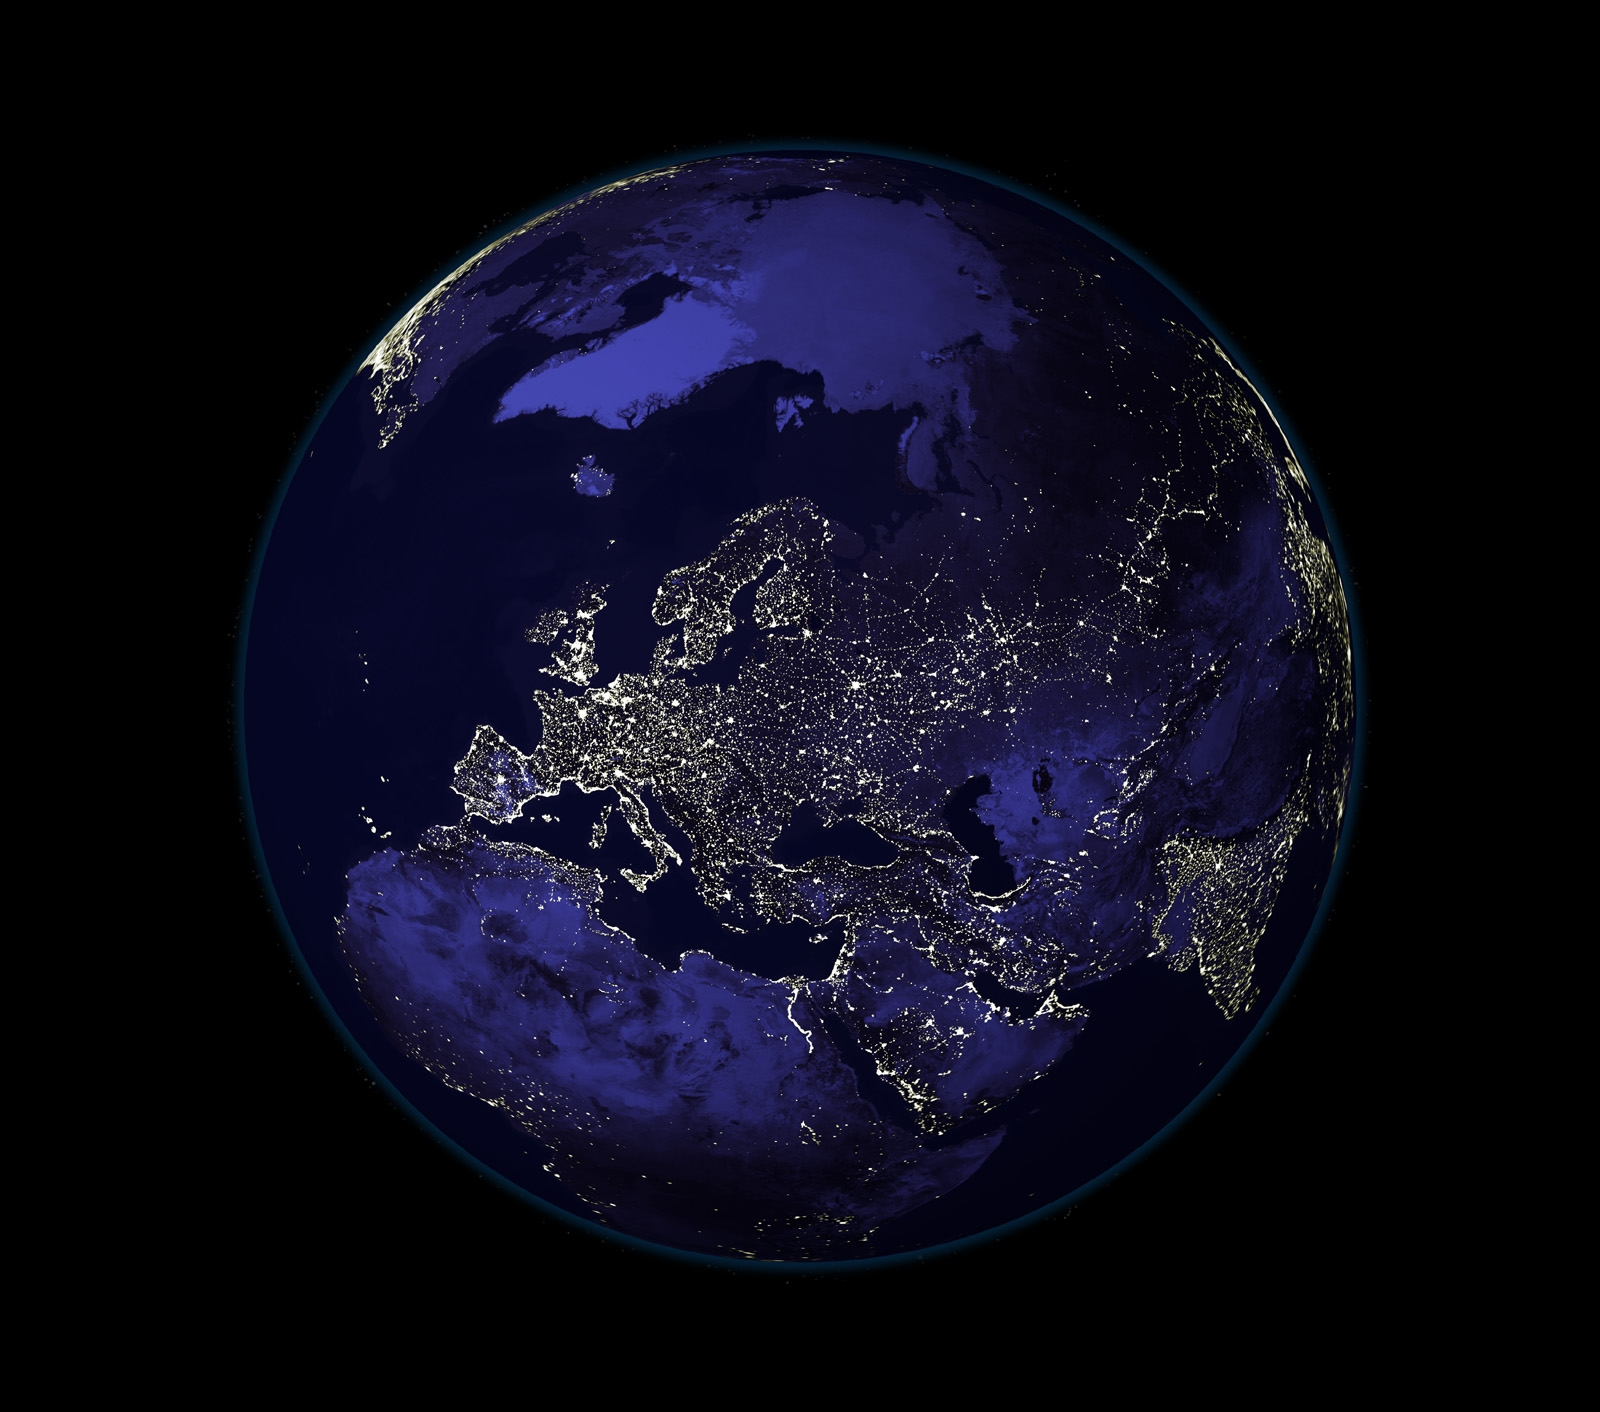
\includegraphics[width=\textwidth]{Tellus}
	\end{subfigure}
\end{figure}

Figure \ref{fig:P:Life} shows how we can constrain the probability of Life.  Our Theory should be able to explain the differences in Figure \ref{fig:Jupiter:Tellus}.

\begin{figure}[H]
	\caption{Rate of abiogenesis in a prebiotic environment as a function of its physical and chemical conditions}\label{fig:P:Life}
	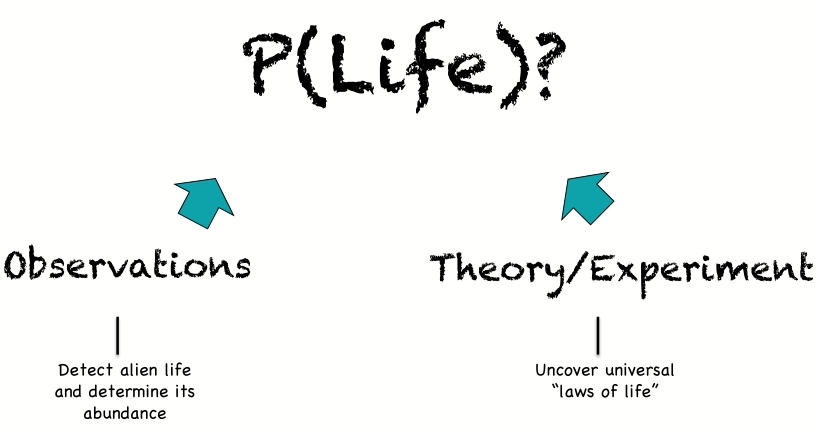
\includegraphics[width=0.9\textwidth]{P_Life}
\end{figure}

''Base metals can be transmuted into gold by stars, and by intelligent beings who understand the processes that power stars, and by nothing else in the universe''--David Deutsch\cite{deutsch2011beginning}.

We want a theory that allows us to understand the diversity of Figure \ref{fig:Earth}.

\section{Exoplanets}

\subsection{The Habitable Zone}

Lecturer: Elizabeth Tasker

Figure \ref{fig:exoplants} shows the number of exoplanets known by discovery technique.\cite{nasa2019Explonet}.

\begin{figure}[H]
	\caption{Exoplanets by discovery technique}\label{fig:exoplants}
	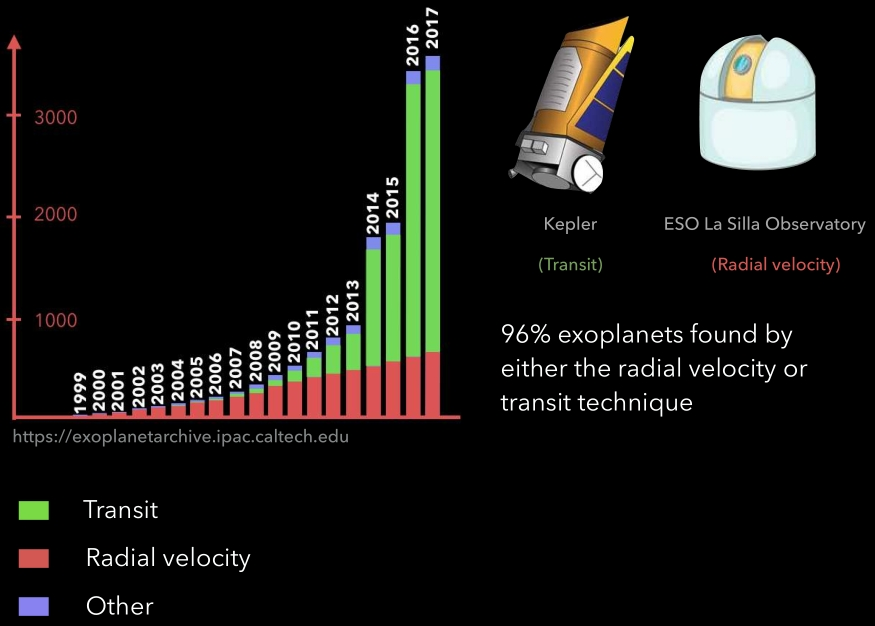
\includegraphics[width=0.9\textwidth]{Exoplanets}
\end{figure}

There are two main techniques:
\begin{itemize}
	\item Radial velocity or Doppler wobble:Orbit with planet causes the
	star to wobble, creating a
	periodic shift in wavelength
	\item Transit: Dip in light as planet crosses
	our line of sight to the star
\end{itemize}

Typically this tells us up to two things about the planet, none of which measurable properties directly relates to surface conditions:
\begin{itemize}
	\item Radius of planet
	\item Mass of planet
\end{itemize}

Our next generation of instruments
aim at atmospheric composition

Rank by most interesting target for habitability

\begin{itemize}
	\item Easiest to recognise Earth-like life 	(water \& carbon-based chemistry)
	\item Needs to be detectable 	(surface water needed)
	\item How much insolation does an 	Earth-like planet need?
\end{itemize}

\begin{figure}[H]
	\caption{Classical Habitable Zone}\label{fig:classical:habitable:zone}
	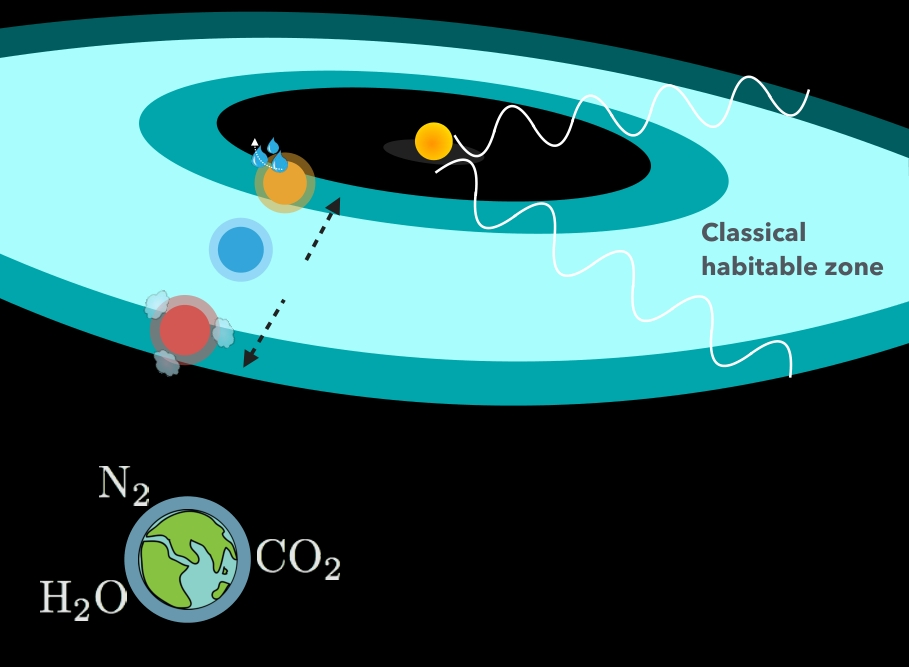
\includegraphics[width=0.9\textwidth]{ClassicalHabitableZone}
\end{figure}

Figure \ref{fig:optimistic:habitable:zone} depicts the Optimistic Habitable Zone, based on empirical data that Venus \& Mars once had surface liquid water 1 - 3.8 Gyrs ago \cite{kasting1993habitable}.
\cite{kopparapu2013habitable}
\begin{figure}[H]
	\caption{Optimistic Habitable Zone }\label{fig:optimistic:habitable:zone}
	    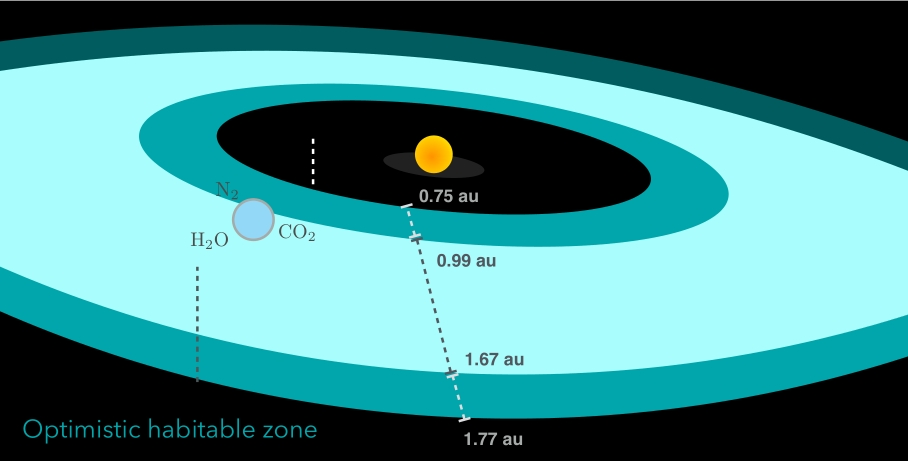
\includegraphics[width=0.9\textwidth]{OptimisticHabitableZone.jpg}
\end{figure}

The classical habitable zone is only for an Earth-like planet. Different planets might have a habitable zone at a different location, or not at all.

Are the exoplanets in Figure \ref{fig:are:these:earthlike} Earth-like? We don’t know. Can only say: If we found another habitable Earth-like planet, it would be in the habitable zone.

\begin{figure}
	\caption{Are these exoplanets Earth-like?}\label{fig:are:these:earthlike}
	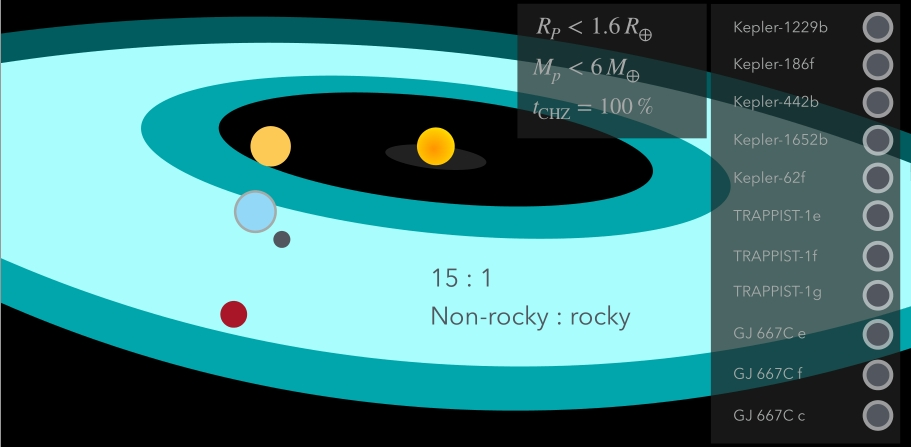
\includegraphics[width=0.9\textwidth]{AreTheseEarthlike}
\end{figure}

Conclusions

\begin{itemize}
	\item We’ve discovered thousands of exoplanets, many of which are similar in
	size to the Earth.
	\item But at the moment, we have no way of knowing what their surfaces are
	like (note that the Earth and Venus are both “Earth-sized planets”.)
	\item Our next generation of telescopes will be able to detect the atmosphere
	of these worlds and tell us something about their surfaces for the first
	time.
	\item The habitable zone is a useful concept for selecting planets for the 	new telescopes, but it offers no guarantee that a planet is habitable.
\end{itemize}

See also \cite{fujii2018exoplanet} and \cite{villanueva2015unique}.

\subsection{Exoplanet Atmospheric Characterization}

Lecturer: Yuka Fujii

Exoplanet Discovery usually come with Size (mass and/or radius) and Orbit--Figure \ref{fig:discovered:exoplanets}.

\begin{figure}[H]
	\caption{Discovered Exoplanets}\label{fig:discovered:exoplanets}
	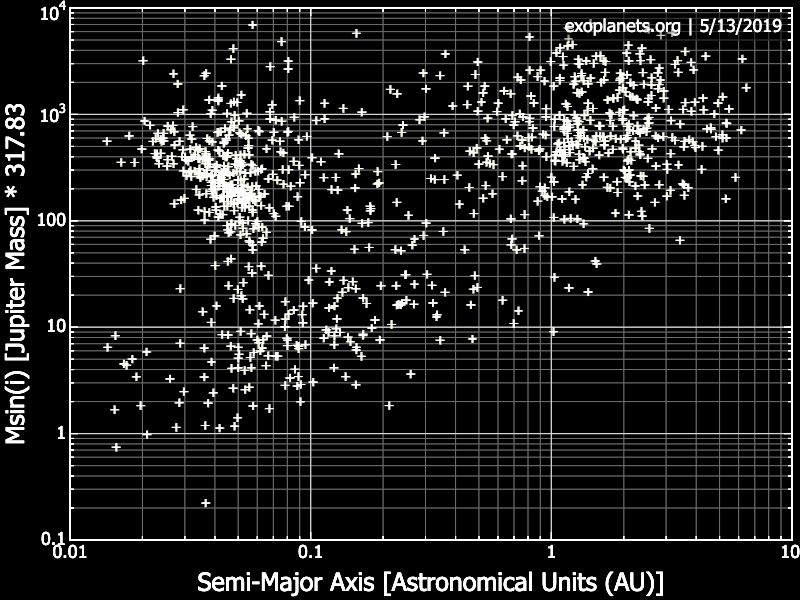
\includegraphics[width=0.9\textwidth]{ExoplanetCharacteristics}
\end{figure} 

Figure \ref{fig:spectrum:earth:twin} depicts the spectrum that we'd expect from a twin planet for Earth. At shorter wavelengths the planet scatters light--Figure \ref{fig:spectrum:earth:twin1}--and the spectrum depends on the composition of the surface; at longer wavelengths it emits infrared--Figure \ref{fig:spectrum:earth:twin2}-- and the spectrum depends on the temperature structure. Figure \ref{fig:spectrum:earth:twin3} depicts the effect of absorption by atmospheric species. For an Earth twin we'd expect to find biologically important molecules. We can scan the plant's surface as it rotates.

\begin{figure}[H]
	\caption{Spectrum of an earth twin}
	\begin{subfigure}[b]{0.45\textwidth}
		\caption{Spectrum of an earth twin}\label{fig:spectrum:earth:twin}
		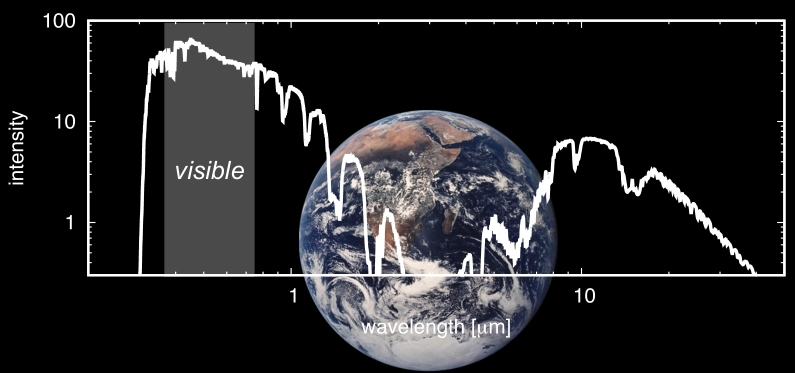
\includegraphics[width=\textwidth]{SpectrumEarthTwin}
	\end{subfigure}
	\begin{subfigure}[b]{0.45\textwidth}
		\caption{At shorter wavelengths the planet scatters light}\label{fig:spectrum:earth:twin1}
		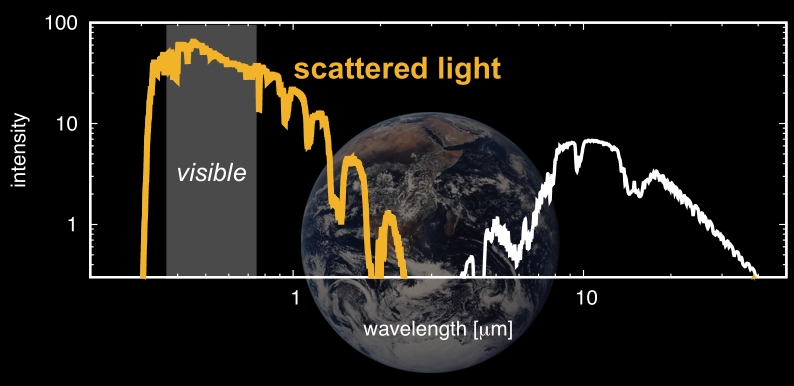
\includegraphics[width=\textwidth]{SpectrumEarthTwin1}
	\end{subfigure}
	\begin{subfigure}[b]{0.45\textwidth}
		\caption{At longer wavelengths it emits infrared}\label{fig:spectrum:earth:twin2}
		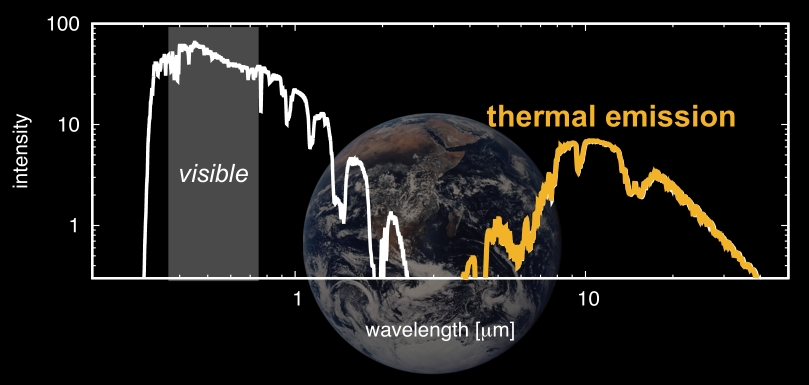
\includegraphics[width=\textwidth]{SpectrumEarthTwin2}
	\end{subfigure}
	\begin{subfigure}[b]{0.45\textwidth}
		\caption{Absorption by atmospheric species}\label{fig:spectrum:earth:twin3}
		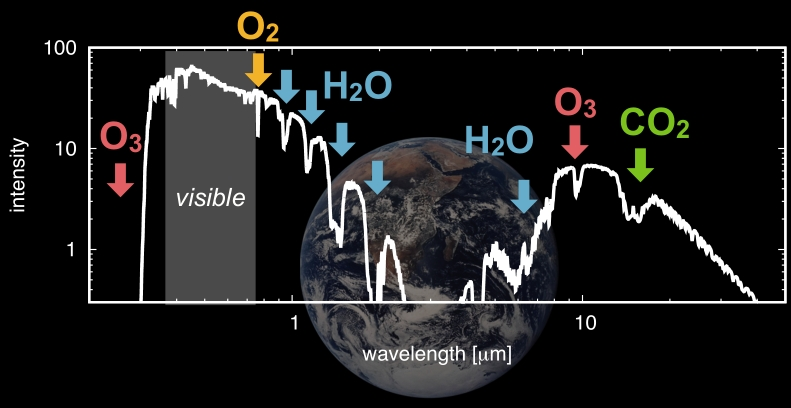
\includegraphics[width=\textwidth]{SpectrumEarthTwin3}
	\end{subfigure}
\end{figure}

Of course it is difficult to disentangle the light of the planet from the star--Figure \ref{fig:StarIsMuchBrighter}. We need to subtract the light of the star.

\begin{figure}[H]
	\caption{Unfortunately the star is many orders of magnitude brighter than its planets}\label{fig:StarIsMuchBrighter}
	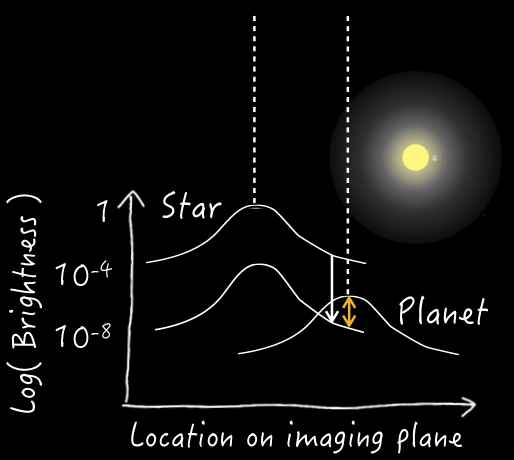
\includegraphics[width=\textwidth]{StarIsMuchBrighter}
\end{figure}

In the past decade, Direct Imaging has been successful with young hot Jupiters in wide orbits--Figure \ref{fig:young:jupiter}. See  Figures  \ref{fig:young:jupiter1}\cite{marois2010images} and Figure \ref{fig:young:jupiter2}
\cite{greenbaum2018gpi}. These planets, however, are an order of magnitude brighter than earthlike planets.

\begin{figure}[H]
	\caption{Success with Young Jupiter-like Planets in Distant Orbits}\label{fig:young:jupiter}
	\begin{subfigure}[b]{0.45\textwidth}
		\caption{}\label{fig:young:jupiter1}
		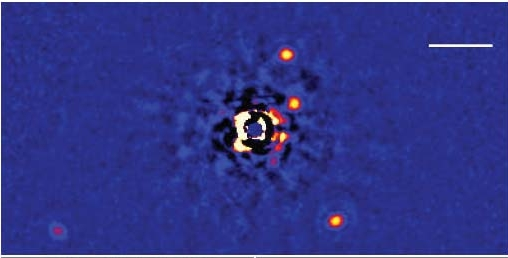
\includegraphics[width=\textwidth]{DirectImaging1.jpg}
	\end{subfigure}
	\begin{subfigure}[b]{0.45\textwidth}
		\caption{}\label{fig:young:jupiter2}
		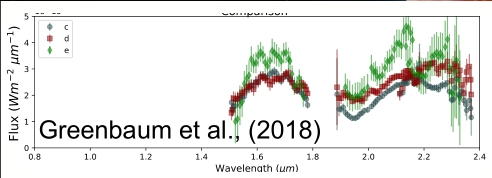
\includegraphics[width=\textwidth]{DirectImaging2.jpg}
	\end{subfigure}
\end{figure}

The discovery of transiting planets has opened up new prospects for studying exoplanet spectra--Figure \ref{fig:transiting:planets} without special instruments. A transiting planet is one that passes in front of the Star because its orbital plane is aligned with the telescope--Figure \ref{fig:transiting:planets2}. A small portion of the light is filtered through the planetary atmosphere--Figure \ref{fig:transiting:planets3}.
\begin{figure}[H]
	\caption{Transiting Planets}\label{fig:transiting:planets}
	\begin{subfigure}[t]{0.3\textwidth}
		\caption{}\label{fig:transiting:planets1}
		
\includegraphics[width=\textwidth]{TransitingPlanets1}
	\end{subfigure}
	\begin{subfigure}[t]{0.3\textwidth}
		\caption{Passing in front}\label{fig:transiting:planets2}
		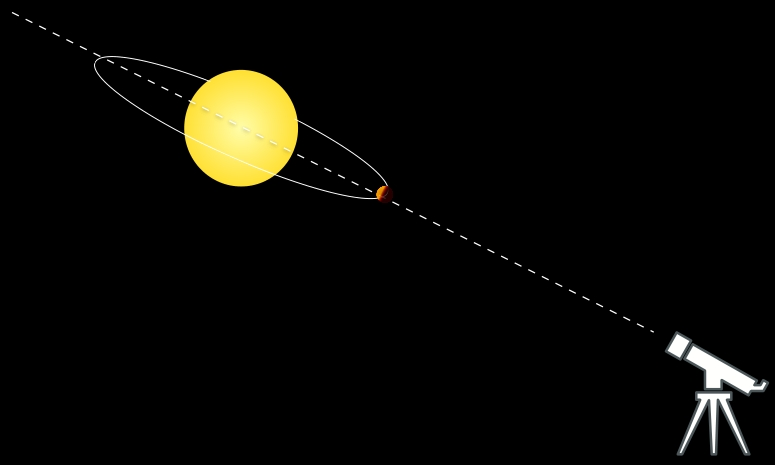
\includegraphics[width=\textwidth]{TransitingPlanets2}
	\end{subfigure}
	\begin{subfigure}[t]{0.3\textwidth}
		\caption{Transmission Spectroscopy}\label{fig:transiting:planets3}
		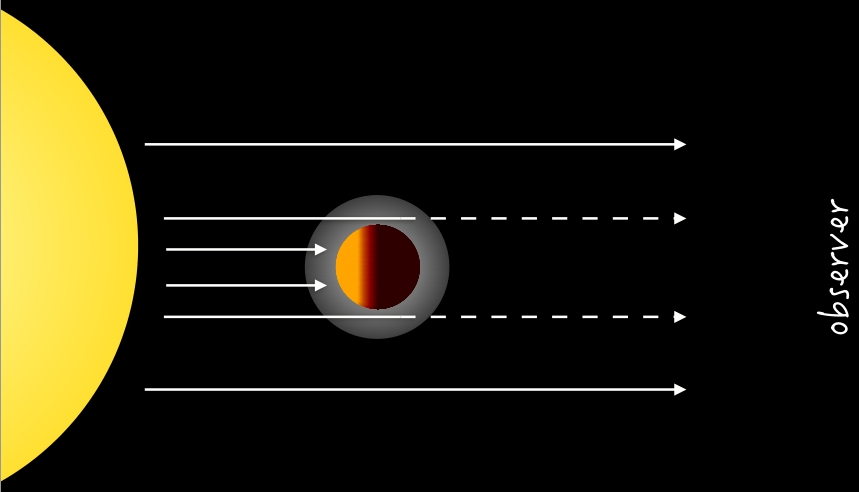
\includegraphics[width=\textwidth]{TransitingPlanets3}
	\end{subfigure}
\end{figure}
	

Summary: Key observations to characterize atmospheres (and surfaces) of exoplanets
\begin{itemize}
	\item Direct Imaging
	\item  Transmission spectroscopy
	\item  Secondary eclipse
	\item  Phase curves
\end{itemize}
Using these techniques, how would you find life on an Earth-twin?

\cite{sagan1993search}
\cite{kaltenegger2017characterize}
\cite{fujii2018exoplanet}

\cite{robinson2011earth}

\cite{deming2013infrared}
\cite{knutson2007map}

\section{What is Life?}

\subsection{Constraining the Definition of Life}

Lecturer:  Sara Imari Walker

''... living matter, while not eluding the laws of physics as established up to date, is likely to involve other laws of physics hitherto unknown''\cite{schrodinger1944life}

\begin{figure}[H]
	\caption{History of Unifications in Physics}
	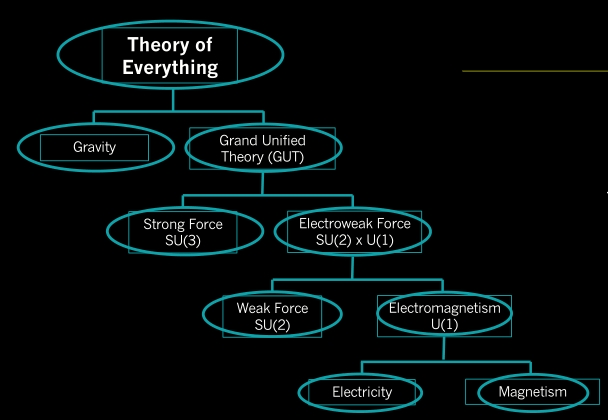
\includegraphics[width=0.9\textwidth]{Unifications}
\end{figure}
''The theory of everything is a theory of everything except of those things that theorize''--David Krakauer.

Examples of "Life"
\begin{itemize}
	\item The Cell as a unit of Life--Figure \ref{fig:cell}
	\item Metabolism--Figure \ref{fig:metabolism}
	\item Tardigrade--an extremophile that can live in space--Figure \ref{fig:tardigrade}. Maybe we should think about the widest set of conditions under which life \textit{can} exist.
	\item Two-headed planarian worms--Figure \ref{fig:2headed:planaria}. What is the limit for viable life?\cite{levin2019planarian}
	\item What is we replace RNA/DNA with XNA?
	\item We can consider scales of organization, as with Social Insects--Figure \ref{fig:social:insects}. Is the super-organism, the colony, "alive"? Is life something that emerges in chemistry, but can exist at higher levels?\cite{pratt2015psychology}
	\item Is a City alive--Figure \ref{fig:city}?
	\item Is there life on the scale of the Planet\cite{lovelock1974atmospheric}--Figure \ref{fig:gaia}?
\end{itemize}

\begin{figure}[H]
	\caption{The Cell as a unit of Life}\label{fig:cell}
	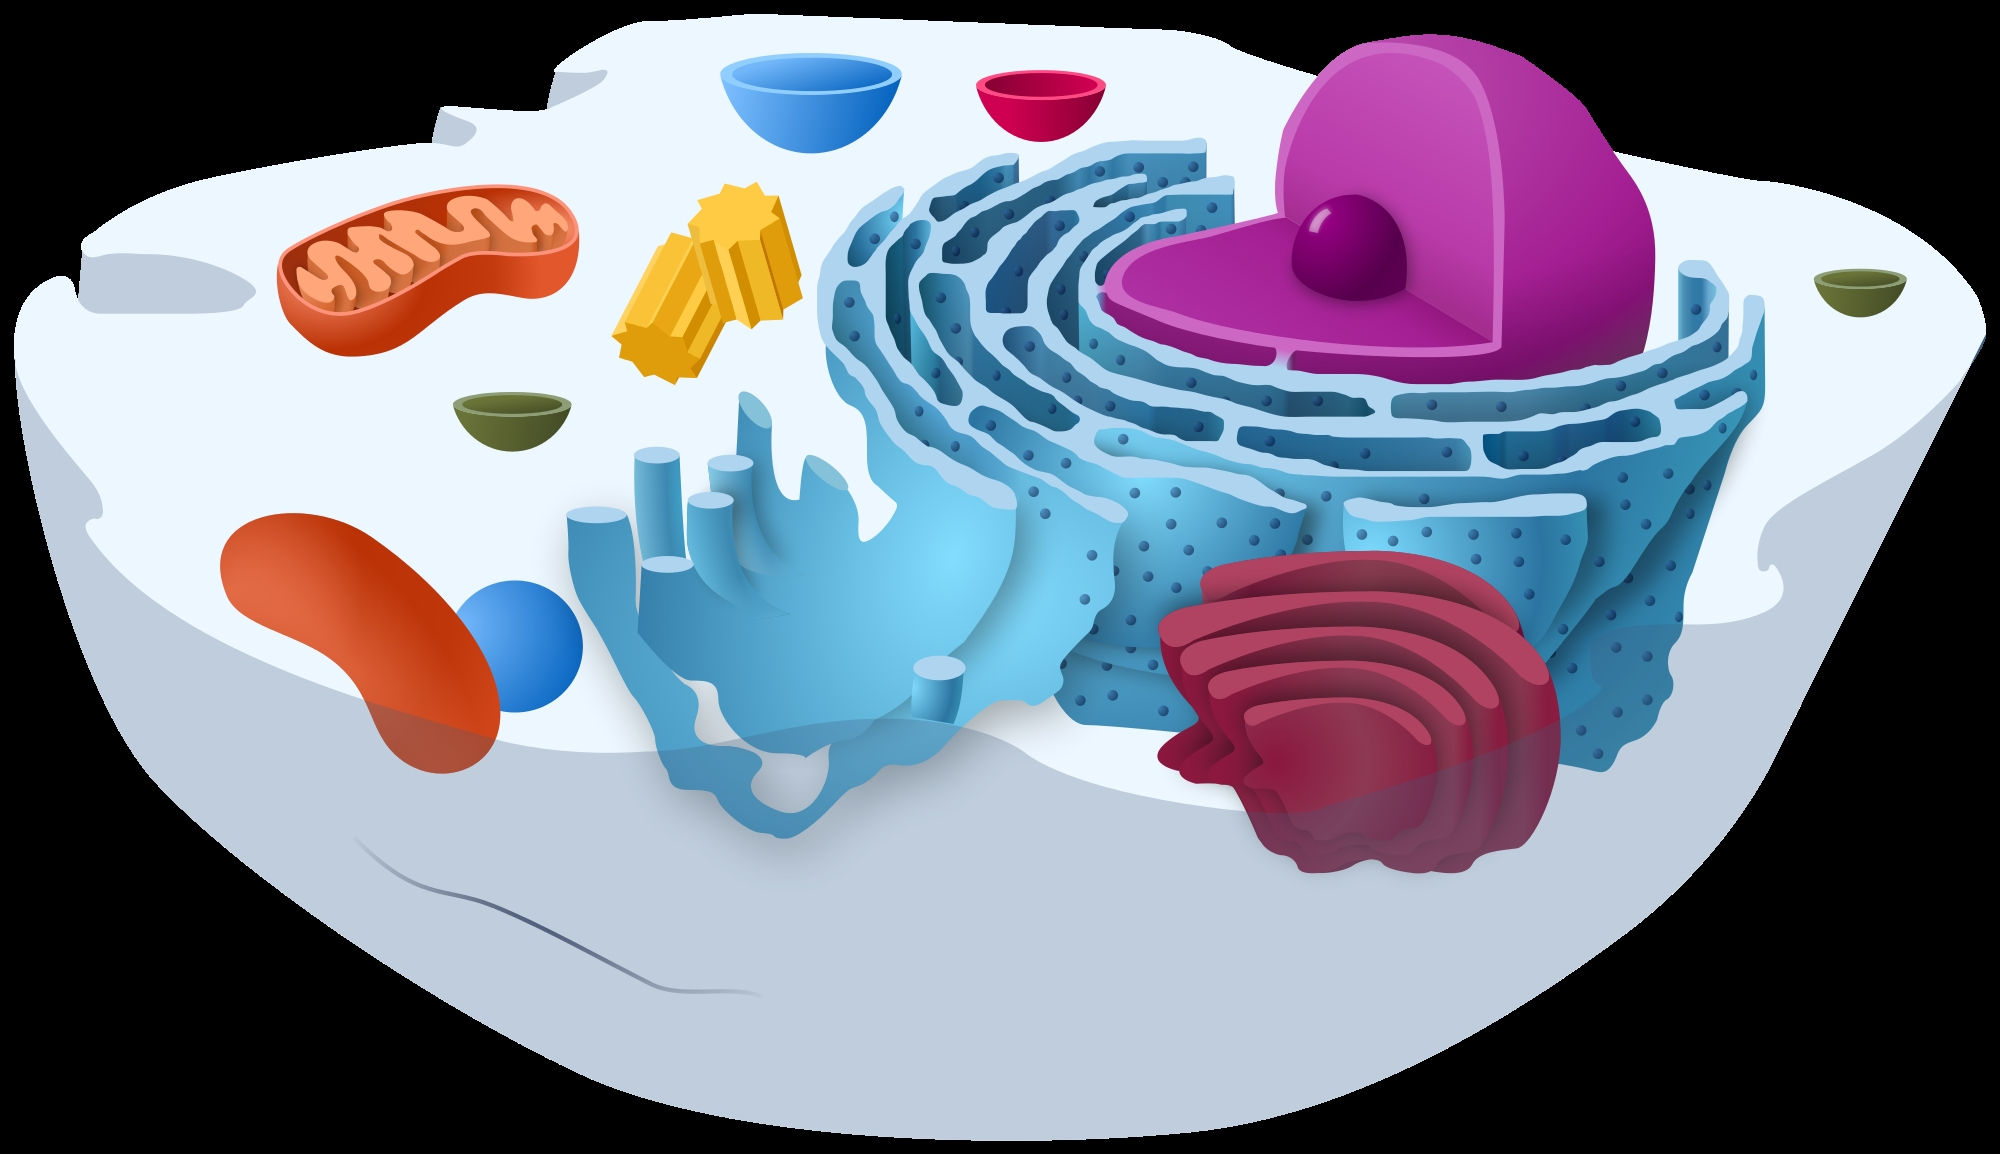
\includegraphics[width=0.9\textwidth]{Cell}
\end{figure}

\begin{figure}[H]
	\caption{Metabolism}\label{fig:metabolism}
	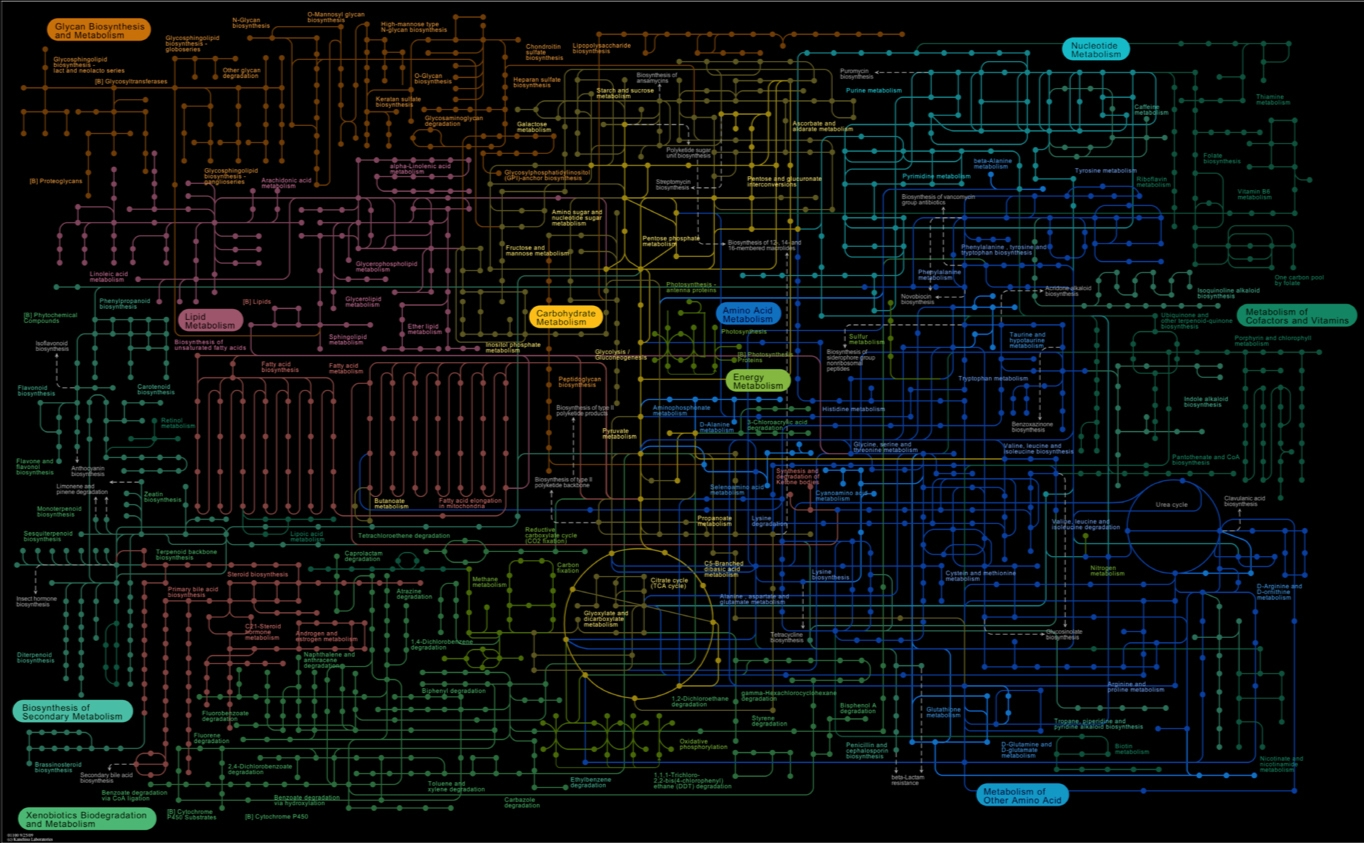
\includegraphics[width=0.9\textwidth]{Metabolism}
\end{figure}

\begin{figure}[H]
	\caption{Tardigrade--an extremophile that can live in space}\label{fig:tardigrade}
	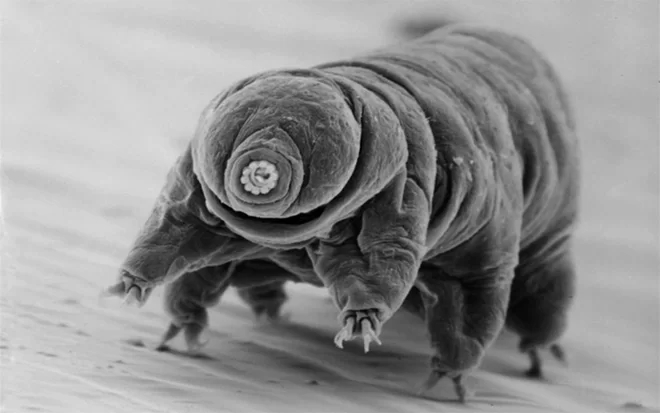
\includegraphics[width=0.9\textwidth]{Tardigrade}
\end{figure}


\begin{figure}[H]
	\caption{Two Headed Planaria}\label{fig:2headed:planaria}
	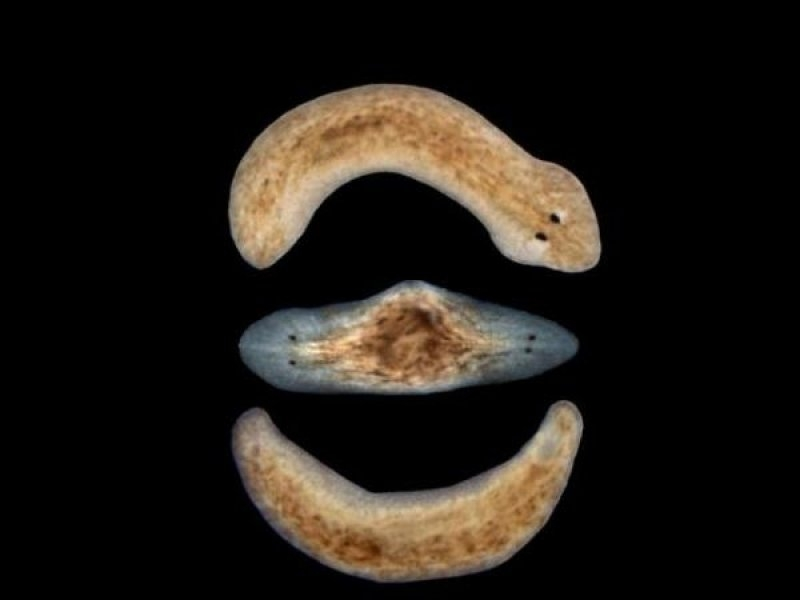
\includegraphics[width=0.9\textwidth]{TwoHeadedPlanaria}
\end{figure}

\begin{figure}[H]
	\caption{Social Insects: is the super-organism "alive"?}\label{fig:social:insects}
	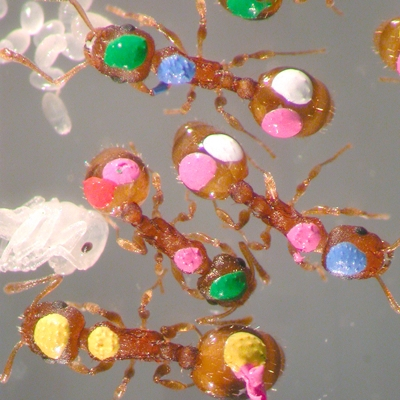
\includegraphics[width=0.9\textwidth]{SocialInsects}
\end{figure}

\begin{figure}[H]
	\caption{City}\label{fig:city}
	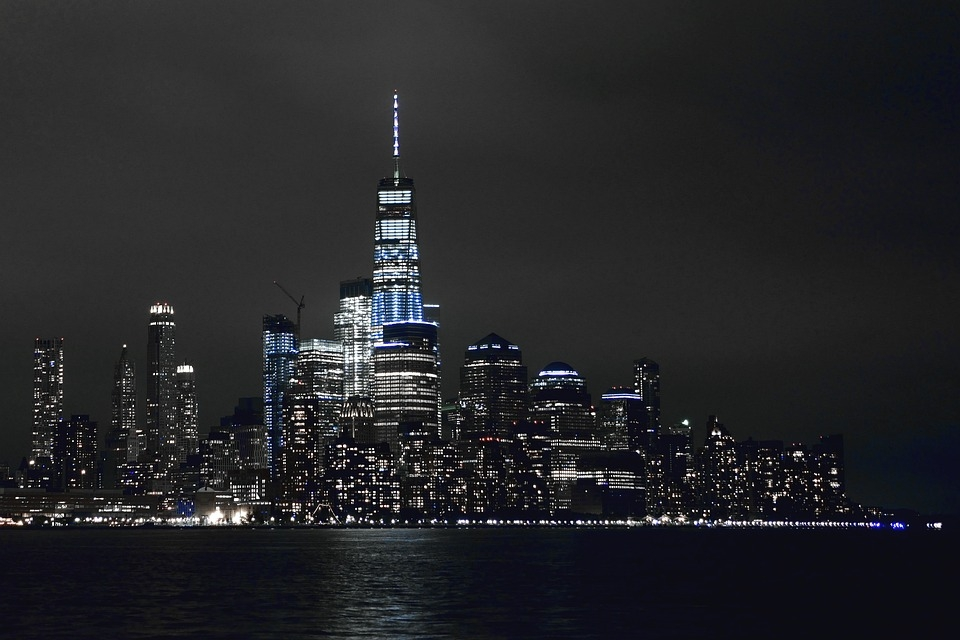
\includegraphics[width=0.9\textwidth]{City}
\end{figure}

\begin{figure}[H]
	\caption{Is there Life on the scale of a Planet?}\label{fig:gaia}
	\begin{subfigure}[b]{0.45\textwidth}
		\caption{Gaia}
		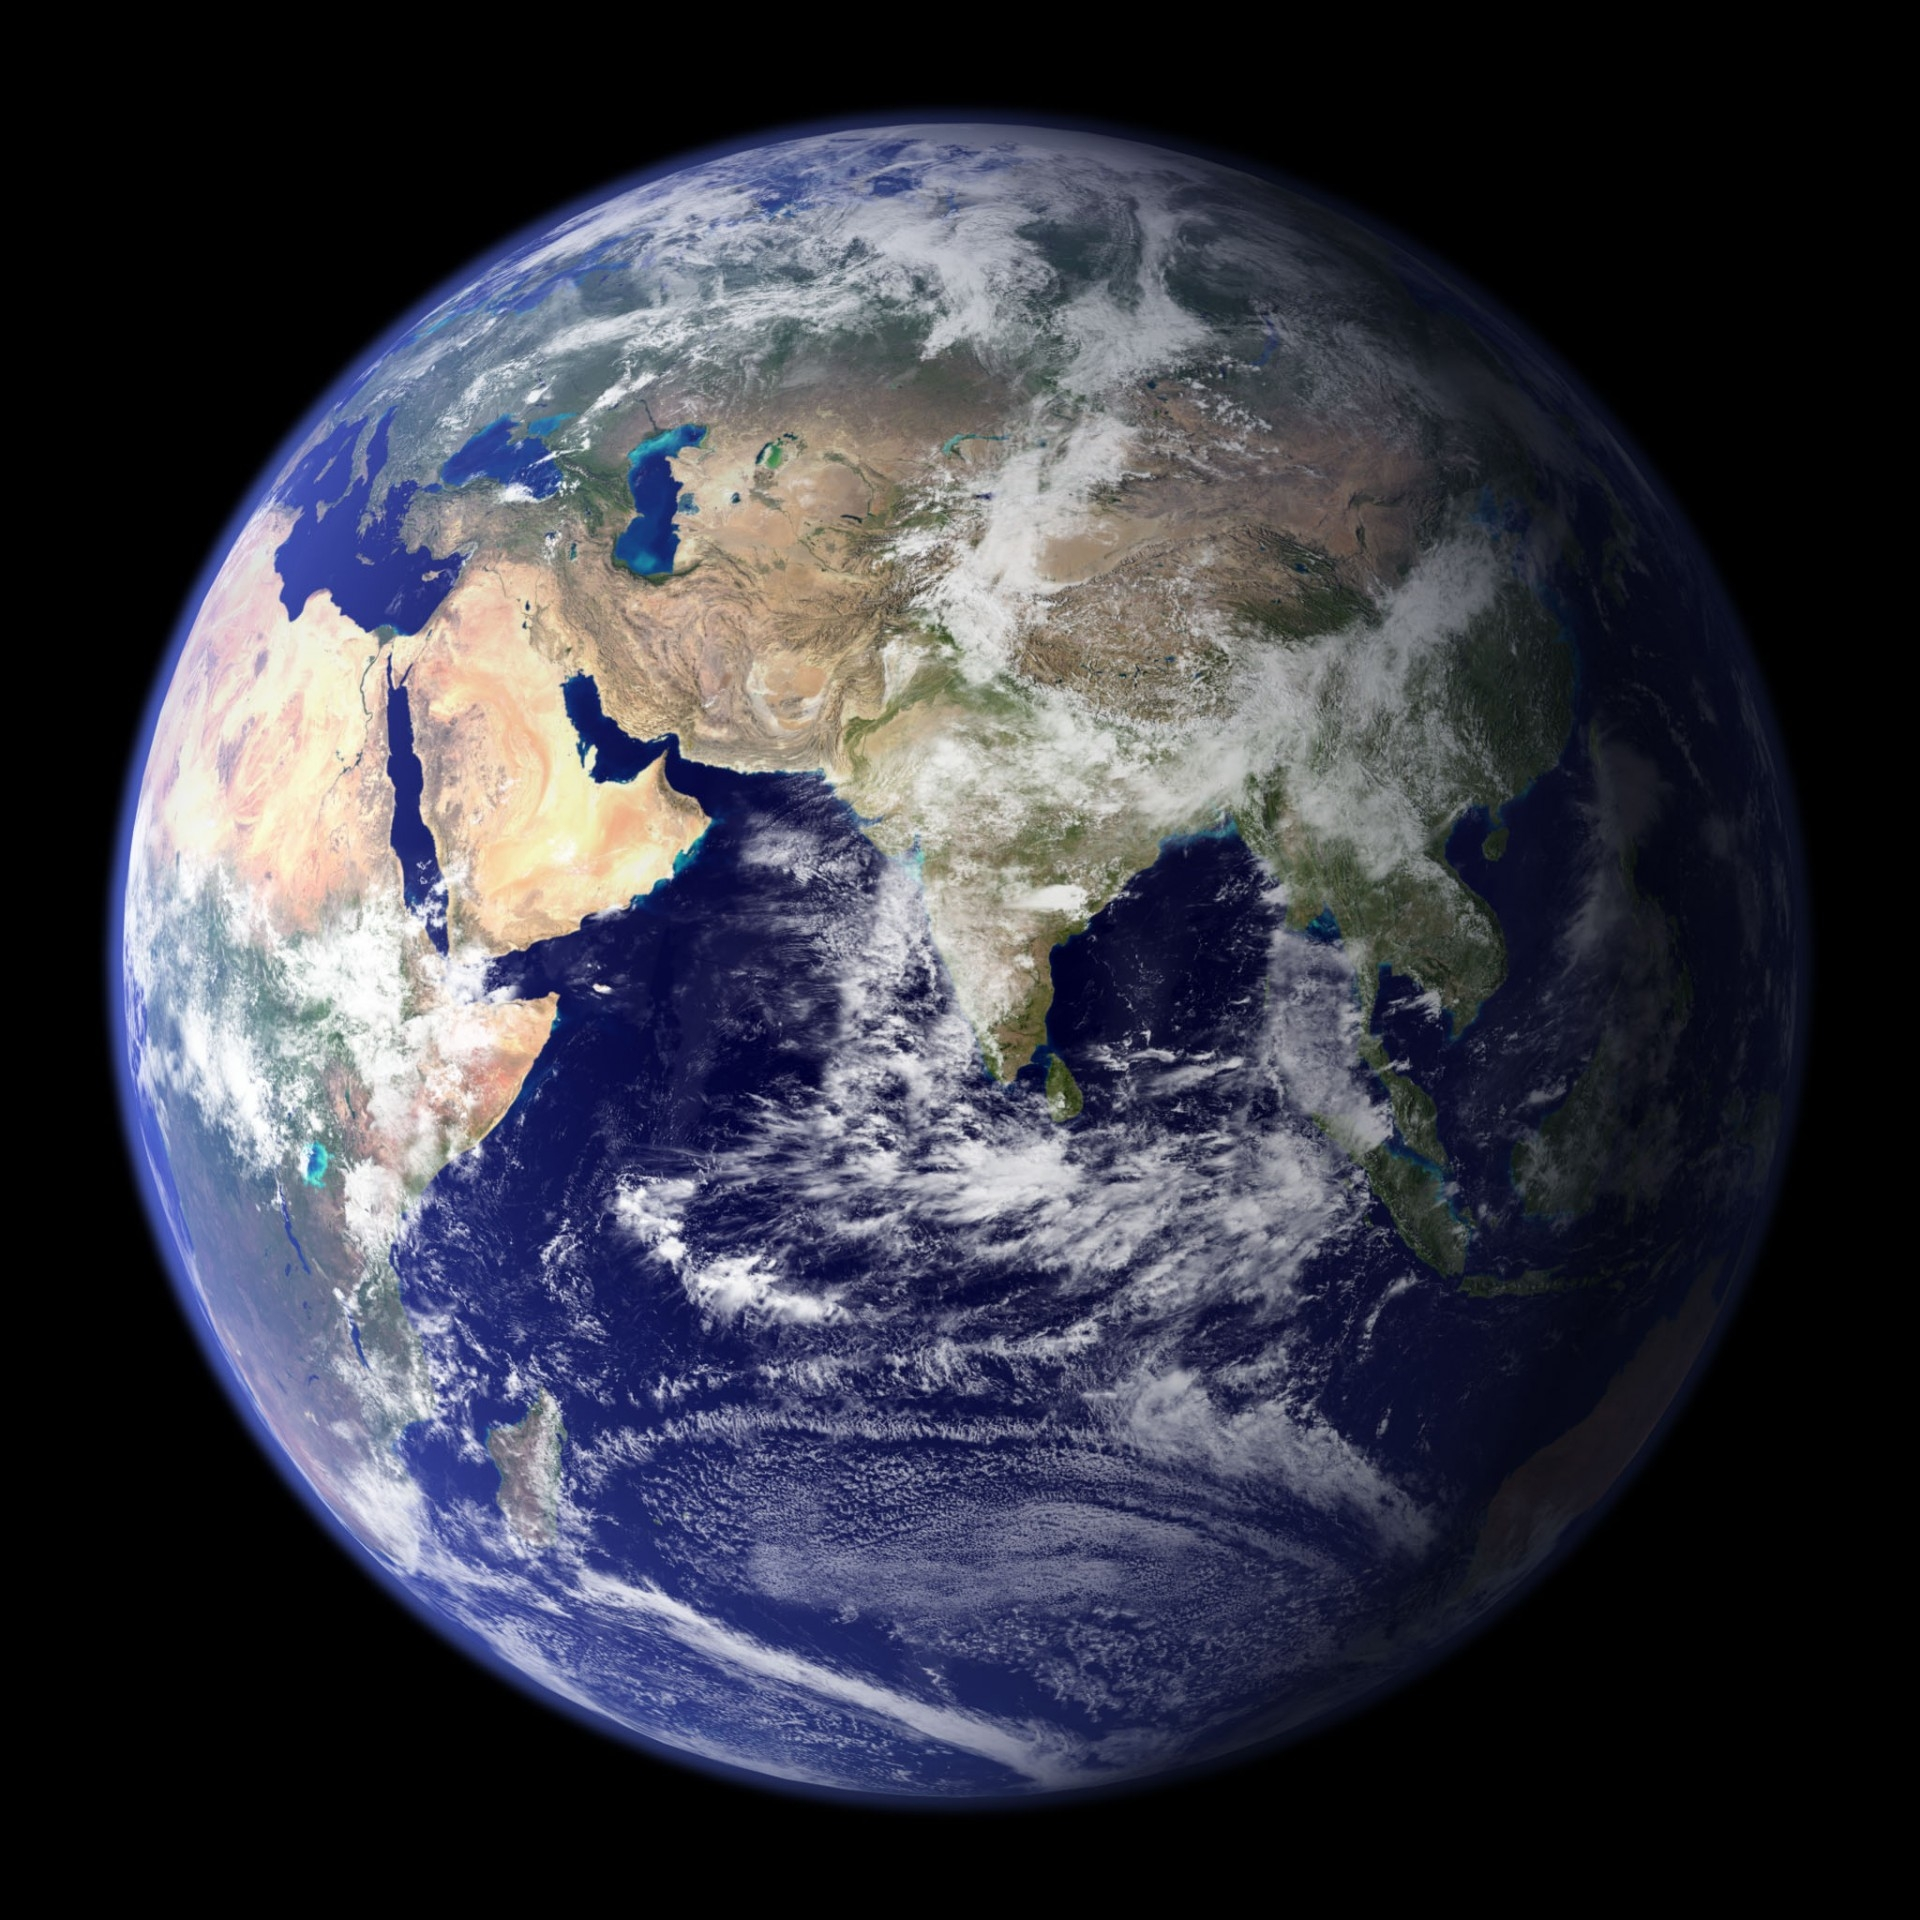
\includegraphics[width=\textwidth]{Globe1}
	\end{subfigure}
	\begin{subfigure}[b]{0.45\textwidth}
		\caption{Network representation of the global inventory of
			enzymatically catalyzed biochemical reactions}
		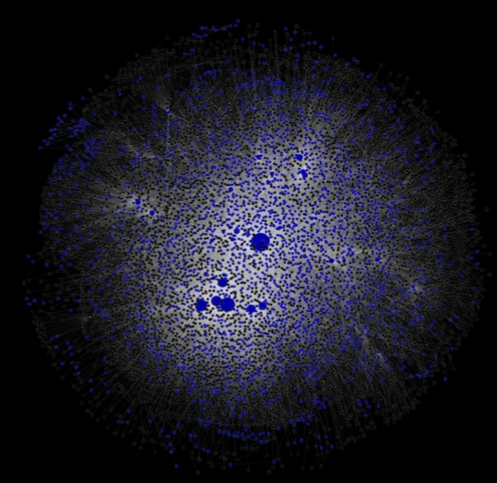
\includegraphics[width=\textwidth]{Globe2}
	\end{subfigure}
\end{figure}


\subsection{Weird Life}

Lecturer: Sarah Maurer

The material in this section is entirely speculative.

\begin{itemize}
	\item No Cells--diffusion systems. But it is very restrained: have to get the right values for parameters.
	\item Membrane-less Cells? Organization of 	chemical gradients\cite{hollants2011life}\cite{kim2001life}
	\begin{itemize}
		\item Mineral surfaces
		\item Coacervates
		\item Oil droplets
		\item Aerosols
	\end{itemize}
	\item No water? 
	\begin{itemize}
		\item Polar solvents\cite[Chapter 6]{board2007limits}--Figure \ref{fig:no:water}. Water, ammonia, and sulphuric acid can:
			\begin{itemize}
				\item drive formation of carbon-carbon bonds;
				\item hydrogen bond.
			\end{itemize}
		\item Non-polar solvents\cite{cejkova2014dynamics}--Figure \ref{fig:non:polar}.
	\end{itemize}
	\item No liquid?\cite[Chapter 6]{board2007limits}
	\begin{itemize}
		\item Solids
		\begin{itemize}
			\item Ices?
			\item Very slow metabolic rates (longer time scales)
		\end{itemize}
		\item Gases
		\begin{itemize}
			\item Higher temperatures
			\item Less stable large molecules
			\item Much larger (galaxy level?)
		\end{itemize}
	\end{itemize}
\end{itemize}


\begin{figure}[H]
	\caption{No Water? Polar solvents}\label{fig:no:water}
	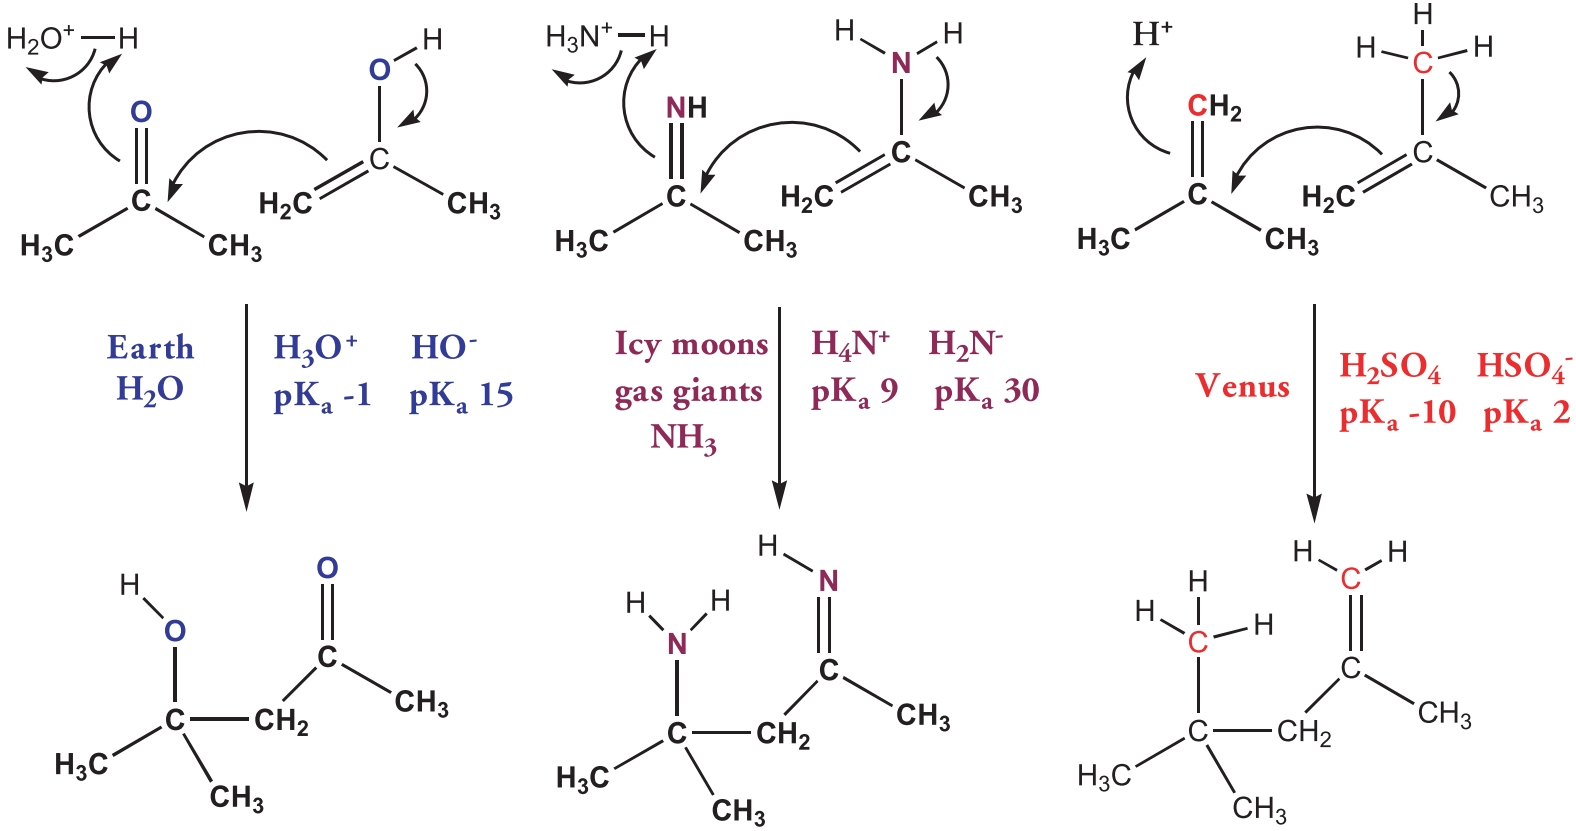
\includegraphics[width=0.9\textwidth]{NoWater}
\end{figure}

\begin{figure}[H]
	\caption{No water? Non-polar solvents}\label{fig:non:polar}
	\begin{subfigure}[t]{0.5\textwidth}
		\caption{Titan--liquid ethane/methane--very cold}
		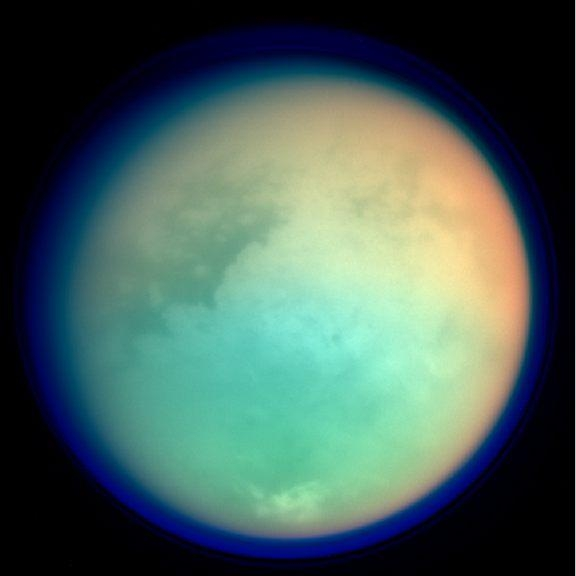
\includegraphics[width=\textwidth]{Titan}
	\end{subfigure}
	\begin{subfigure}[t]{0.5\textwidth}
		\caption{Io--liquid sulfur--Hotter than Earth}
		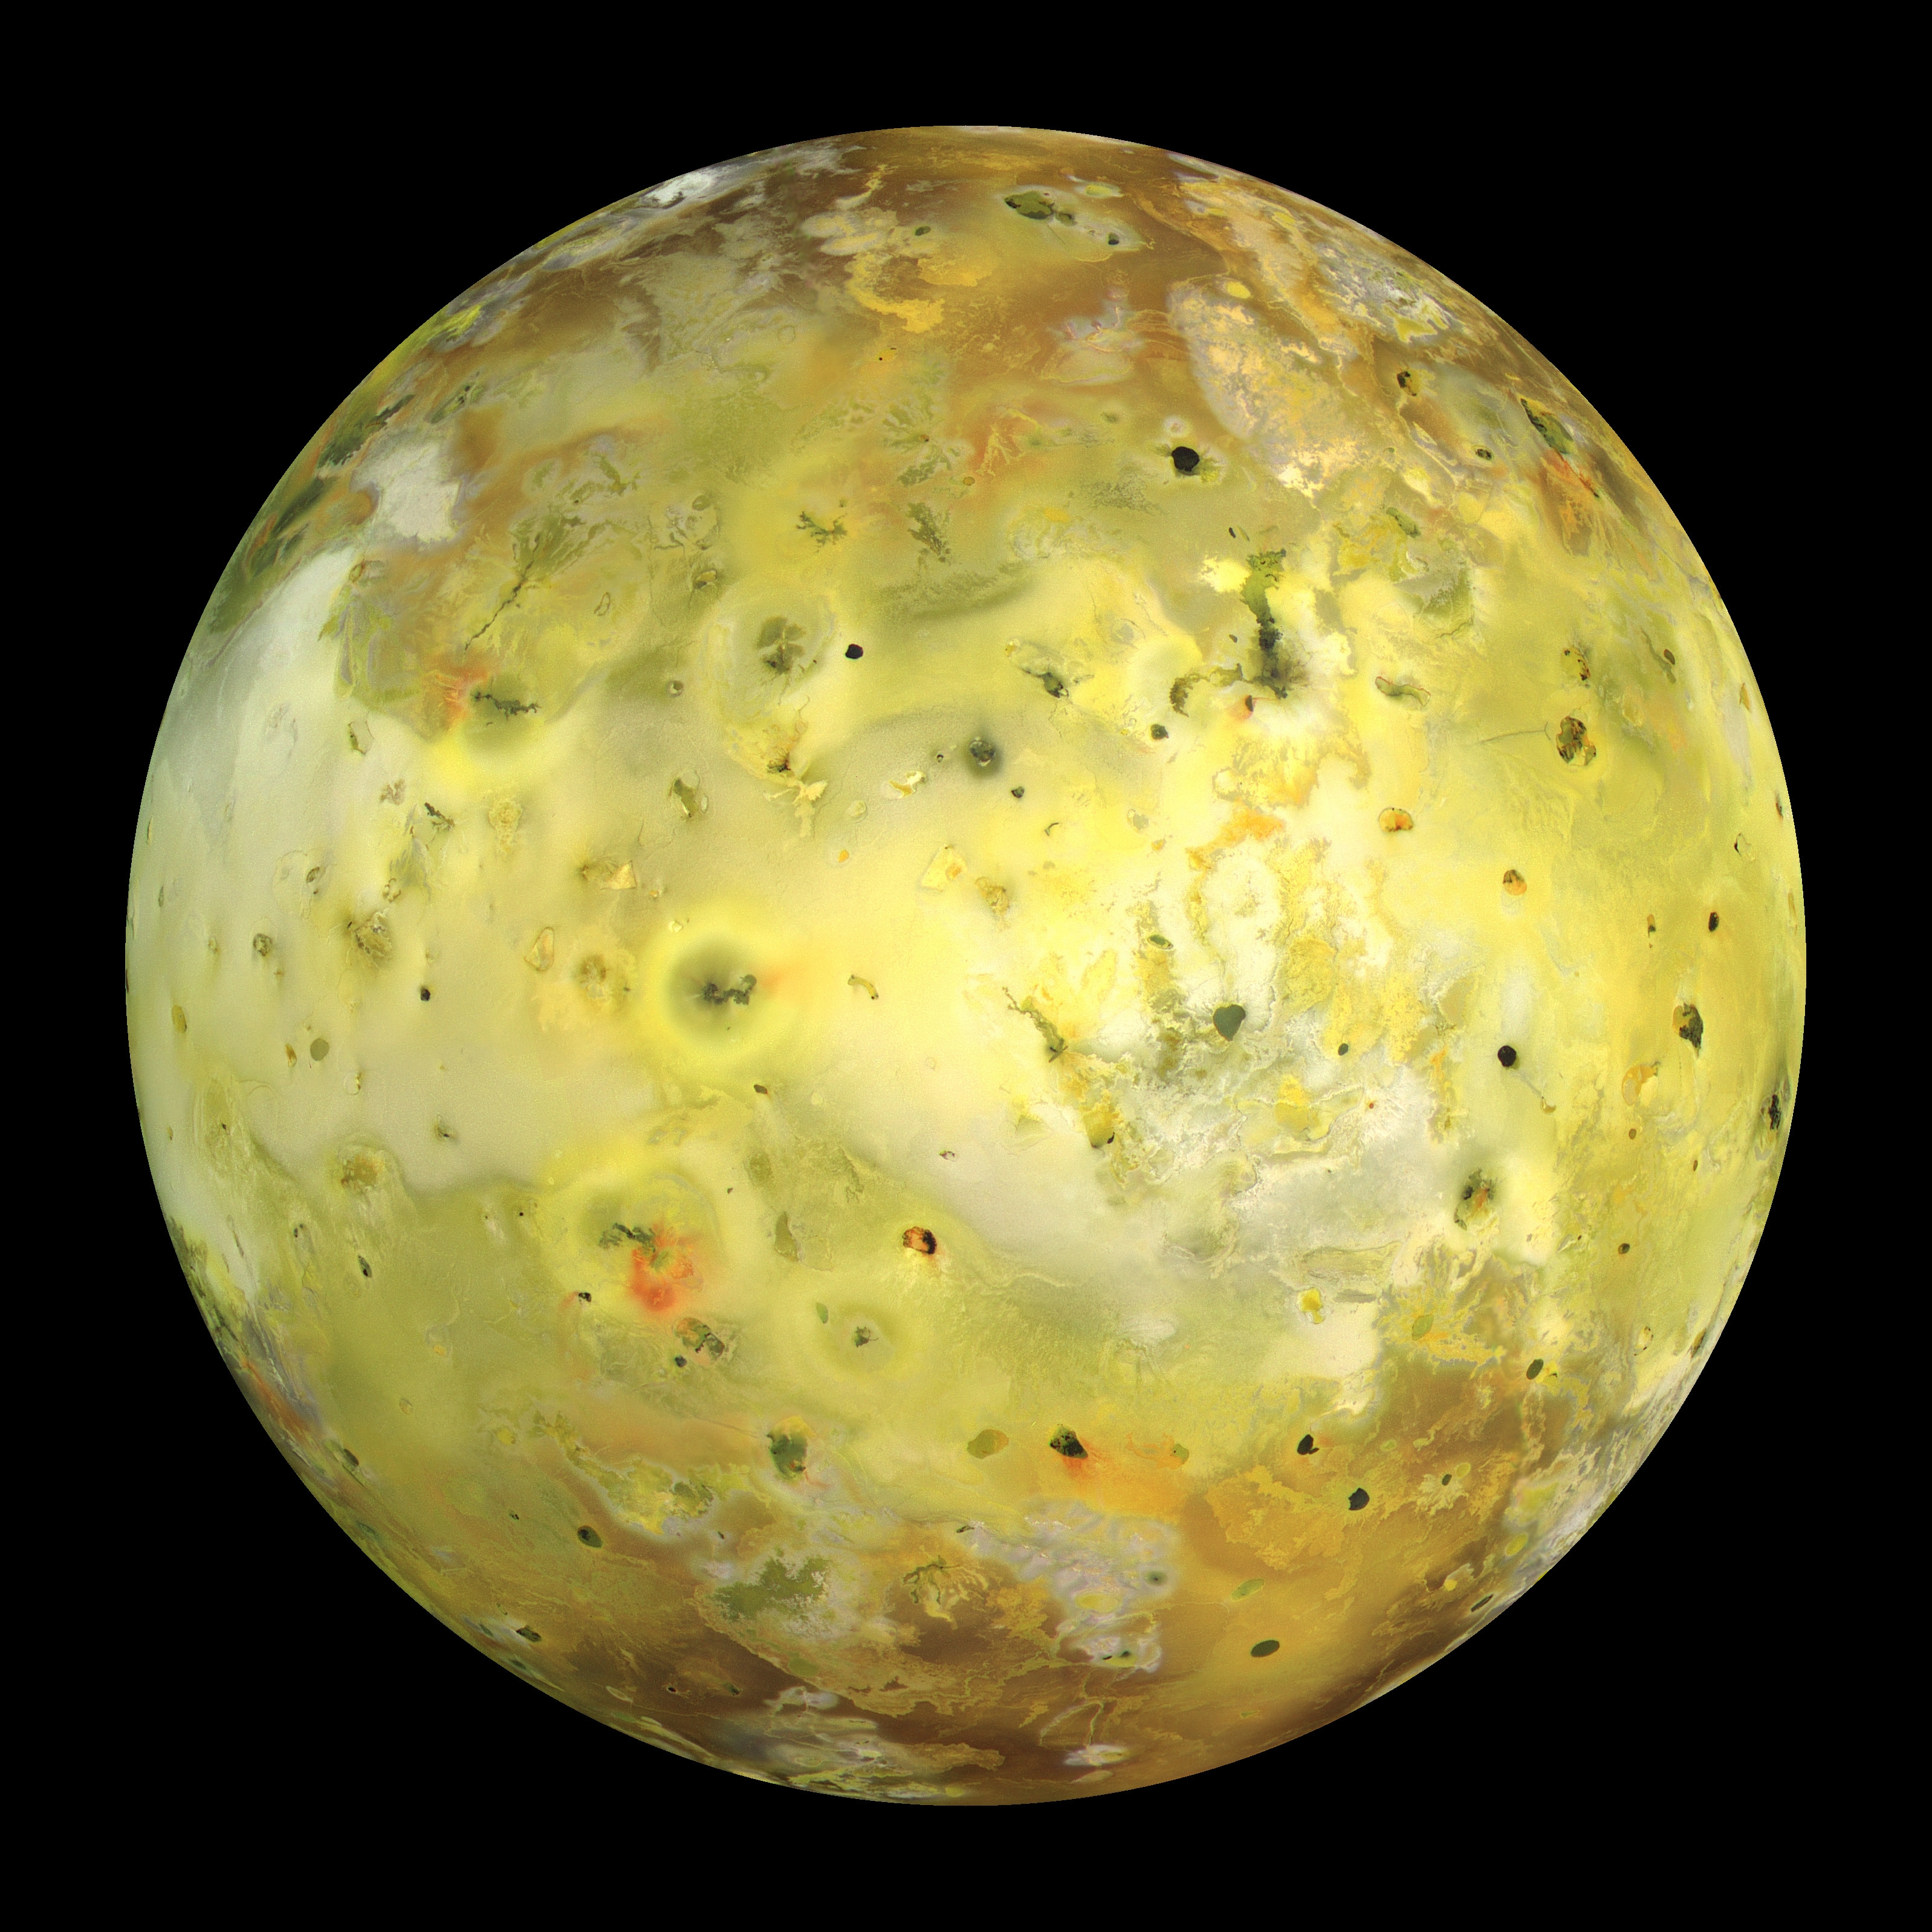
\includegraphics[width=\textwidth]{Io}
	\end{subfigure}
\end{figure}

Open Questions

\begin{itemize}
	\item What other substrates could life exist in?
	\item Would we recognize it?
\end{itemize}



\section{Abstract and general Models for Life}

Lecturer: Sara Imari Walker

See discussion in \cite{trifonov2011vocabulary}. We want a general definition so we can recognize and explain life elsewhere in the Universe.

Theory vs. Model vs. Definition (ad hoc, based on Life On earth). We are limited by a single example of life--Figure \ref{fig:yatol}--descended from the \gls{gls:LUCA}. \gls{gls:LUCA} would have had DNA, translation, proteins, cellular organization: it doesn't take us back to the origin of life on Earth.

\begin{figure}[H]
	\caption{We are limited by a single example of life}\label{fig:yatol}
	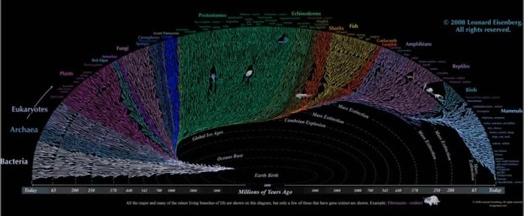
\includegraphics[width=\textwidth]{YATOL}
\end{figure}

Genetics-First versus Metabolism-First--Figure \ref{fig:GeneticsVsMetabolism}.

\begin{itemize}
	\item Genetics-First, e.g. RNA World
	\item Metabolism-First, e.g. autocatalytic sets
\end{itemize}

\begin{figure}[H]
	\caption{Genetics-First versus Metabolism-First: Two competing hypotheses}\label{fig:GeneticsVsMetabolism}
	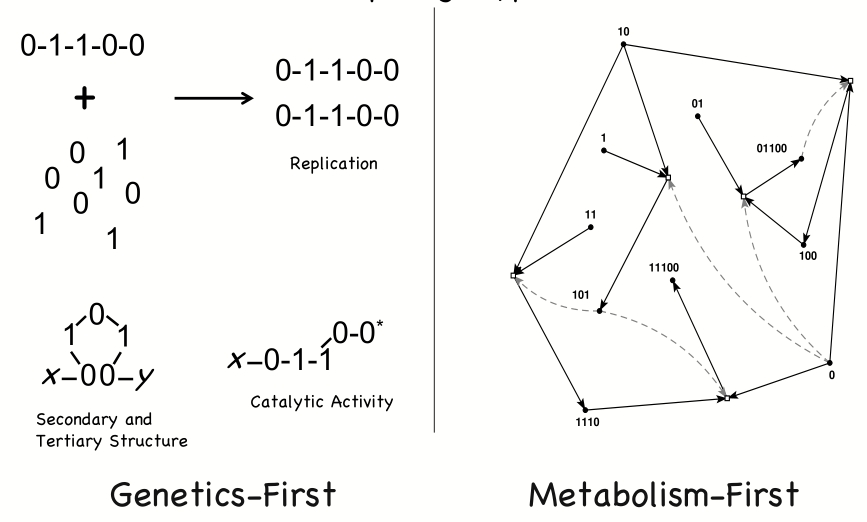
\includegraphics[width=0.9\textwidth]{GeneticsVsMetabolism}
\end{figure}

Figure \ref{fig:GeneticsVsMetabolism} puts these two points of view side-by-side. We need Theories, not just Models: the Definition needs to come from Theory, not from a Model.

Life as an information processing system--\cite{nurse2008life}

''Focusing on information… may perhaps provide our best shot at uncovering universal laws of life that work not just for biological systems with known chemistry but also for putative artificial and alien life.''--\cite{cronin2016beyond}--Figure \ref{fig:LifeInformation}.

\begin{figure}[H]
	\caption{Life as Information}\label{fig:LifeInformation}
	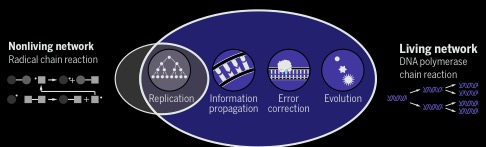
\includegraphics[width=0.9\textwidth]{LifeInformation}
\end{figure}


\section{The Multiple Origins of Life}

Lecturer: David Krakauer

\subsection{The Argument}

\begin{itemize}
	\item Origin of Life Research is dominated by Naturalist-reductionists.
	\begin{itemize}
		\item My car and my adding machine 	understand nothing: they are
		not in that line of business--John Searle
	\end{itemize}
	\item an alternative would be Functionalists (like AI before Turing and modern ML)
	\begin{itemize}
		\item We are not interested in the fact that the brain has the consistency of cold porridge--Alan Turing.
	\end{itemize}
	\item Life emerges from an adaptive arrow of time (the reverse of the thermodynamic arrow).
	\item The Adaptive arrow of time is multi-scale and applies as readily to inference as organic evolution (this is not dependent on biological chemistry)
	\item The key to any form of adaptive evolution is the Agent, AKA, the Individual
	\item Individuals have evolved countless times in earth history - emerging from
	forms both ecological and individual: e.g. Virus evolution and the Block Chain.
\end{itemize}

\subsection{Reversing the Arrow of Time}

\begin{itemize}
	\item[Thermodynamic arrow] ''Let us draw an arrow arbitrarily. If as we follow the arrow we find more and more
	of the random element in the state of the world, then the arrow is pointing towards
	the future; if the random element decreases the arrow points towards the past … I
	shall use the phrase “time's arrow” to express this one-way property of time which
	has no analogue in space''--Arthur Eddington\cite{eddington1939philosophy}
	
	\item[Adaptive arrow]''It was Darwin’s chief contribution, not only to Biology but to the whole of natural science, to have brought to light a process by which contingencies a priori
	improbable are given, in the process of time, an increasing probability, until it is their non-occurrence, rather than their occurrence, which becomes highly improbable.''--Ronald Fisher\cite{fisher1930genetical}
\end{itemize}

\begin{figure}[H]
	\caption{Thermodynamic Arrow of Time wants to roll down hill, Adaptive up hill towards lower probability.}\label{fig:NaturalSelection}
	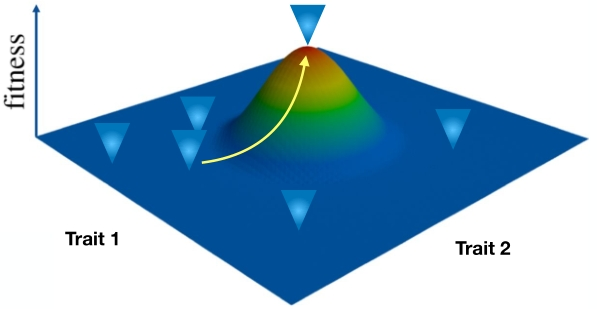
\includegraphics[width=0.9\textwidth]{NaturalSelection}
\end{figure}

\subsection{The Theory of the Adaptive Arrow of Time}

\begin{itemize}
	\item The Fundamental Theorem of Natural Selection
	R.A. Fisher, 1930
	\item ''adaptation is an optimization dynamics
	transferring information
	from the environment into the agent
	- reducing uncertainty about states of the world''\cite{rockmore2018cultural}
	\item A scale-invariant, substrate-neutral, stochastic process
	\begin{itemize}
		\item Evolution
		\item Inference
		\item Learning
	\end{itemize}
\end{itemize}

\subsection{Evolutionary Agents}

Sol Spiegelman wanted to know what was the minimal genome for \textit{Q Beta Phage}. He bred 74 generations in the presence of \textit{QBeta RNA replicase}, which it would normally have to synthesize--Figure \ref{fig:SpiegelmanMonster}. The RNA reduces from 4500 base pairs to 218!\cite{spiegelman1965synthesis}
\begin{figure}[H]
	\caption{The Spiegelman Monster}\label{fig:SpiegelmanMonster}
	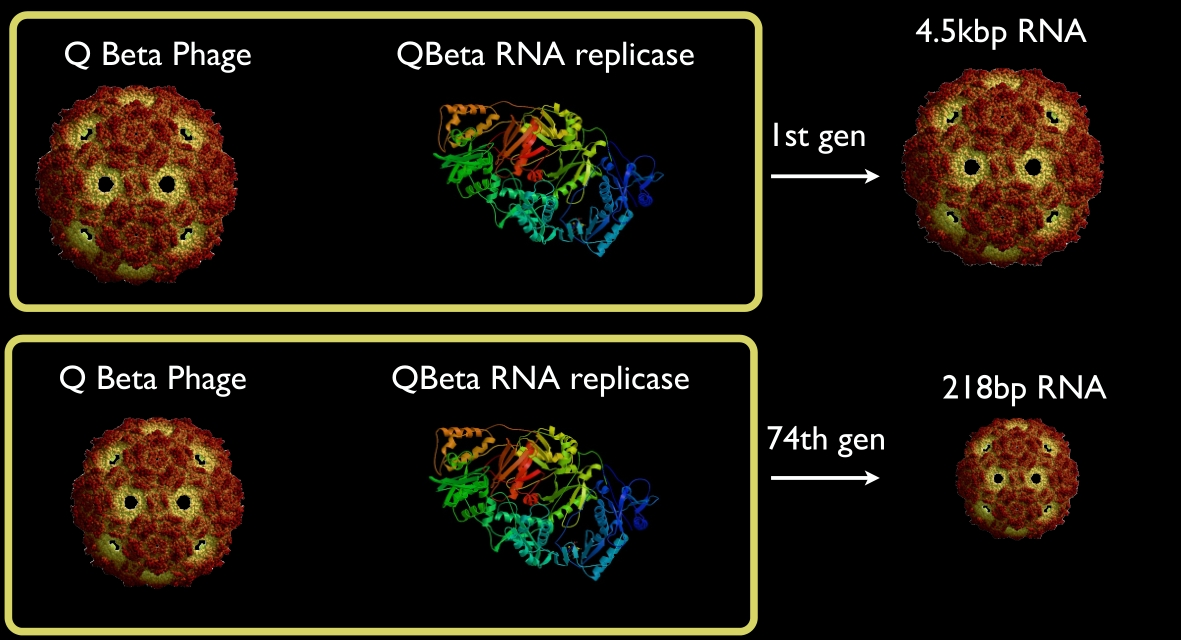
\includegraphics[width=0.9\textwidth]{SpiegelmanMonster}
\end{figure}

Figure \ref{fig:SpiegelmanMonsterVenn} depicts the process: $v_i$ represents the information held by the virus only, $h_i$ the information held by the host (environment), and $s_i$ the information that is shared. The virus eliminates the shared information if the information is always there! If we don't know that the information is always there, we get autonomy.

\begin{figure}[H]
	\caption{Elimination of shared Information}\label{fig:SpiegelmanMonsterVenn}
	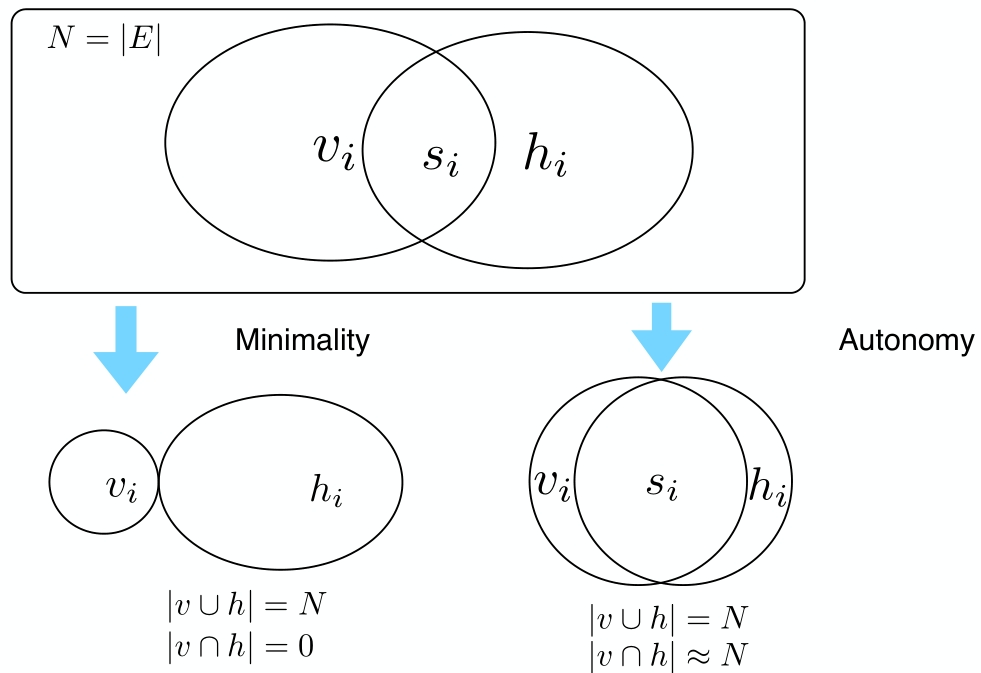
\includegraphics[width=0.9\textwidth]{SpiegelmanMonsterVenn}
\end{figure}

 Virus is normally considered as non-living, because it depends its environment, but we depend on our environment too, e.g. for vitamins. There is a spectrum of adaptive agency--Figure \ref{fig:SpectrumOfLife}.  ''Life is a mechanism for acquiring adaptive information about the World, that it propagates forward in time''. This includes computer viruses and blockchain!
 
\begin{figure}[H]
	\caption{The Spectrum of Life}\label{fig:SpectrumOfLife}
	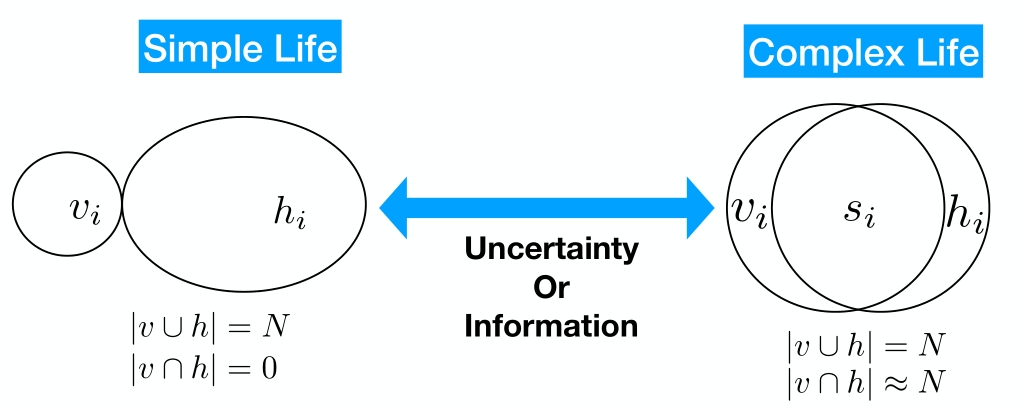
\includegraphics[width=0.9\textwidth]{SpectrumOfLife}
\end{figure}
Open Questions

\begin{itemize}
	\item[Fundamentalists] Are we only interested in the initial necessary conditions for all subsequent life (e.g. Evolveability out of abiotic physics as the most fundamental basis for understanding).
	\item[Pluralists] Or are we interested in the multiple origins of life (adaptive agency) and thereby the many analogous processes that can support these (e.g. 	Coarse-Grained effective theories at multiple scales?)
\end{itemize}
\section{Evolutionary Computation}

\cite{mitchell1998introduction}
\cite{eiben2003introduction}
\cite{holland1992adaptation}
\cite{forrest1993genetic}
\cite{ma2014novo}
\cite{marshall2014evolution}


\section{Scaling}

\cite{anderson2013altered}
\cite{damuth1981population}
\cite{enquist1998allometric}
\cite{enquist2012land}
\cite{marquet2005scaling}
\cite{schmidt1984scaling}
\cite{tucker2014evolutionary}
\cite{west1997general}

\section{Energy}

\cite{odum1976energy}
\cite{odum1983systems}
\cite{schmidt1997animal}
\cite{brown2004toward}
\cite{sibly2012metabolic}
\cite{ernest2003thermodynamic}
\cite{savage2004predominance}
\cite{dell2011systematic}
\cite{kempes2017thermodynamic}

% end of text 

% glossary
\printglossaries

% bibliography go here
 
\bibliographystyle{unsrt}
\addcontentsline{toc}{section}{Bibliography}
\bibliography{origins,wikipedia}

\end{document}
